% Practice 2: Ontologies - AI Fundamentals
% Master in Artificial Intelligence 2025-26
% Santiago Delgado Ferreiro & David Carballo Rodríguez

\documentclass[12pt,a4paper]{article}

% Essential packages
\usepackage[utf8]{inputenc}
\usepackage[english]{babel}
\usepackage{graphicx}
\usepackage{float}
\usepackage{hyperref}
\usepackage{listings}
\usepackage{xcolor}
\usepackage{geometry}
\usepackage{fancyhdr}
\usepackage{titlesec}
\usepackage{enumitem}
\usepackage{caption}
\usepackage{subcaption}


% Page configuration
\geometry{
    top=2.5cm,
    bottom=2.5cm,
    left=3cm,
    right=3cm
}

% Header and footer configuration
\pagestyle{fancy}
\fancyhf{}
\fancyhead[L]{Practice 2: Ontologies}
\fancyhead[R]{AIF 2025-26}
\fancyfoot[C]{\thepage}
\renewcommand{\headrulewidth}{0.4pt}
\renewcommand{\footrulewidth}{0.4pt}

% Hyperlink configuration
\hypersetup{
    colorlinks=true,
    linkcolor=blue,
    filecolor=magenta,      
    urlcolor=cyan,
    pdftitle={Practice 2: Ontologies},
    pdfauthor={Santiago Delgado Ferreiro, David Carballo Rodríguez},
}

% Code listing configuration
\lstdefinelanguage{SPARQL}{
    keywords={PREFIX, SELECT, WHERE, FILTER, OPTIONAL, UNION, GROUP, ORDER, BY, LIMIT, DISTINCT, COUNT, YEAR, ASC},
    keywordstyle=\color{blue}\bfseries,
    string=[s]{"}{"},
    stringstyle=\color{red},
    comment=[l]{\#},
    commentstyle=\color{gray}\itshape,
    morecomment=[s]{/*}{*/},
    sensitive=true,
    basicstyle=\ttfamily\small,
    breaklines=true,
    showstringspaces=false,
    frame=single,
    numbers=left,
    numberstyle=\tiny\color{gray},
    numbersep=5pt,
}

\lstset{
    basicstyle=\ttfamily\small,
    breaklines=true,
    frame=single,
    numbers=left,
    numberstyle=\tiny\color{gray},
}

% Custom title
\title{
    \textbf{AI Fundamentals}\\
    \Large Practice 2: Ontologies\\
    \large Master in Artificial Intelligence\\
    \normalsize Academic Year 2025-26
}

\author{
    Santiago Delgado Ferreiro\\
    \texttt{santiago.delgado@estudiante.uam.es}
    \and
    David Carballo Rodríguez\\
    \texttt{david.carballo@estudiante.uam.es}
}

\date{October 2025}

\begin{document}

% Cover page
\maketitle

\vfill

\begin{center}
\vspace{0.5cm}
\textbf{WebProtégé Username:} santi\_david
\end{center}

\newpage

% Table of contents
\tableofcontents
\newpage

% Configure page numbering
\setcounter{page}{1}

%==============================================================================
% SECTION 1: INTRODUCTION
%==============================================================================
\section{Introduction}

Ontologies are formal representations of knowledge that allow structuring and organizing information in a semantic way. In the context of Artificial Intelligence, ontologies play a fundamental role by providing:

\begin{itemize}
    \item \textbf{Knowledge representation:} Formal structuring of concepts and their relationships.
    \item \textbf{Interoperability:} They facilitate information exchange between heterogeneous systems.
    \item \textbf{Automated reasoning:} They allow inferring new knowledge from existing facts.
    \item \textbf{Knowledge reuse:} They promote the creation of shared knowledge bases.
\end{itemize}

\subsection{Practice Objectives}

The main objectives of this practice are:

\begin{enumerate}
    \item \textbf{Understanding ontology structure} through analysis of the OFFF ontology (Ontology of Fast Food Facts).
    \item \textbf{Editing ontologies} using the WebProtégé tool, adding classes, properties, and instances.
    \item \textbf{Performing SPARQL queries} on knowledge bases available on the Semantic Web (DBpedia).
    \item \textbf{Applying theoretical knowledge} to practical cases related to nutrition and food health.
\end{enumerate}

\subsection{Tools Used}

\begin{itemize}
    \item \textbf{WebProtégé:} Web-based collaborative ontology editor (\url{https://webprotege.stanford.edu/})
    \item \textbf{OFFF:} Fast food ontology that integrates nutritional information
    \item \textbf{SPARQL:} Query language for RDF data
    \item \textbf{DBpedia:} Knowledge base extracted from Wikipedia
\end{itemize}

%==============================================================================
% SECTION 2: OFFF ONTOLOGY EDITING
%==============================================================================
\section{OFFF Ontology Editing}

\subsection{Context: The OFFF Ontology}

The Ontology of Fast Food Facts (OFFF) is a formal representation of knowledge about fast food, developed by UTHealth. This ontology integrates:

\begin{itemize}
    \item Nutritional information of fast food products
    \item Food components (carbohydrates, proteins, fats, vitamins, minerals)
    \item Allergens present in foods
    \item Specific ingredients
    \item Relationships with health outcomes
\end{itemize}

The hierarchical structure of OFFF allows establishing causal relationships between diet quality and various health problems, facilitating the analysis and reasoning about eating habits.

\subsection{Allergen Selection}

For this practice, 10 allergens have been selected from the official list of internationally recognized food allergens (\url{https://en.wikipedia.org/wiki/List_of_allergens}). The selection was based on the following criteria:

\begin{enumerate}
    \item \textbf{Prevalence:} Most common allergens in the general population
    \item \textbf{Severity:} Potential to cause serious allergic reactions
    \item \textbf{Regulation:} Mandatory labeling in multiple jurisdictions
    \item \textbf{Presence in fast food:} Frequency of occurrence in fast food products
\end{enumerate}

\subsubsection{Selected Allergens}

\begin{enumerate}
    \item \textbf{Peanut}
    \begin{itemize}
        \item One of the most common and potentially fatal allergens
        \item Present in oils, sauces, and processed products
        \item Causes anaphylactic reactions in sensitive individuals
    \end{itemize}
    
    \item \textbf{Tree Nuts}
    \begin{itemize}
        \item Includes almonds, walnuts, hazelnuts, cashews, pistachios
        \item Common in salads, desserts, and baked goods
        \item High risk of cross-reactions between different tree nuts
    \end{itemize}
    
    \item \textbf{Milk}
    \begin{itemize}
        \item Most common allergen in young children
        \item Present in dairy products, ice cream, cream sauces, baked goods
        \item Different from lactose intolerance
    \end{itemize}
    
    \item \textbf{Egg}
    \begin{itemize}
        \item Especially egg white (albumin)
        \item Used in mayonnaise, baked goods, breading
        \item Common in breakfast fast food products
    \end{itemize}
    
    \item \textbf{Fish}
    \begin{itemize}
        \item Includes all finned fish
        \item Present in fish sandwiches, salads, sauces
        \item Reactions usually persist throughout life
    \end{itemize}
    
    \item \textbf{Shellfish}
    \begin{itemize}
        \item Includes crustaceans (shrimp, crab, lobster) and mollusks
        \item Common in salads, wraps, ``premium'' options
        \item One of the most common allergies in adults
    \end{itemize}
    
    \item \textbf{Soy}
    \begin{itemize}
        \item Present in vegetable proteins, oils, lecithin
        \item Extensively used in processed products
        \item Common component in vegetarian burgers
    \end{itemize}
    
    \item \textbf{Wheat}
    \begin{itemize}
        \item Contains gluten (allergy-causing protein)
        \item Present in bread, dough, breading, thickeners
        \item Different from celiac disease
    \end{itemize}
    
    \item \textbf{Sesame}
    \begin{itemize}
        \item Increasingly recognized as an important allergen
        \item Present in breads (buns), sauces (tahini), oils
        \item Recently added to the list of major allergens in the USA
    \end{itemize}
    
    \item \textbf{Celery}
    \begin{itemize}
        \item Common allergen in Europe
        \item Used in broths, soups, salads, condiments
        \item Can cause serious reactions even in small amounts
    \end{itemize}
\end{enumerate}

\subsection{Creating Allergen Subclasses}

\subsubsection{Modification Process}

The process of adding the 10 allergens as subclasses of the \texttt{Allergens} class in WebProtégé consisted of:

\begin{enumerate}
    \item \textbf{Navigation to parent class:} Locate the \texttt{Allergens} class in the OFFF class hierarchy
    \item \textbf{Subclass creation:} Use the ``Create subclass'' function (+) for each allergen
    \item \textbf{Nomenclature:} Use English names following OFFF convention (CamelCase or snake\_case as appropriate)
    \item \textbf{Verification:} Check that subclasses appear correctly in the hierarchy
\end{enumerate}

\subsubsection{Resulting Hierarchical Structure}

The created hierarchy is as follows:

\begin{verbatim}
Allergens
|- Peanut
|- TreeNuts
|- Milk
|- Egg
|- Fish
|- Shellfish
|- Soy
|- Wheat
|- Sesame
`- Celery
\end{verbatim}


\subsubsection{Graphical Evidence}

\begin{figure}[H]
    \centering
    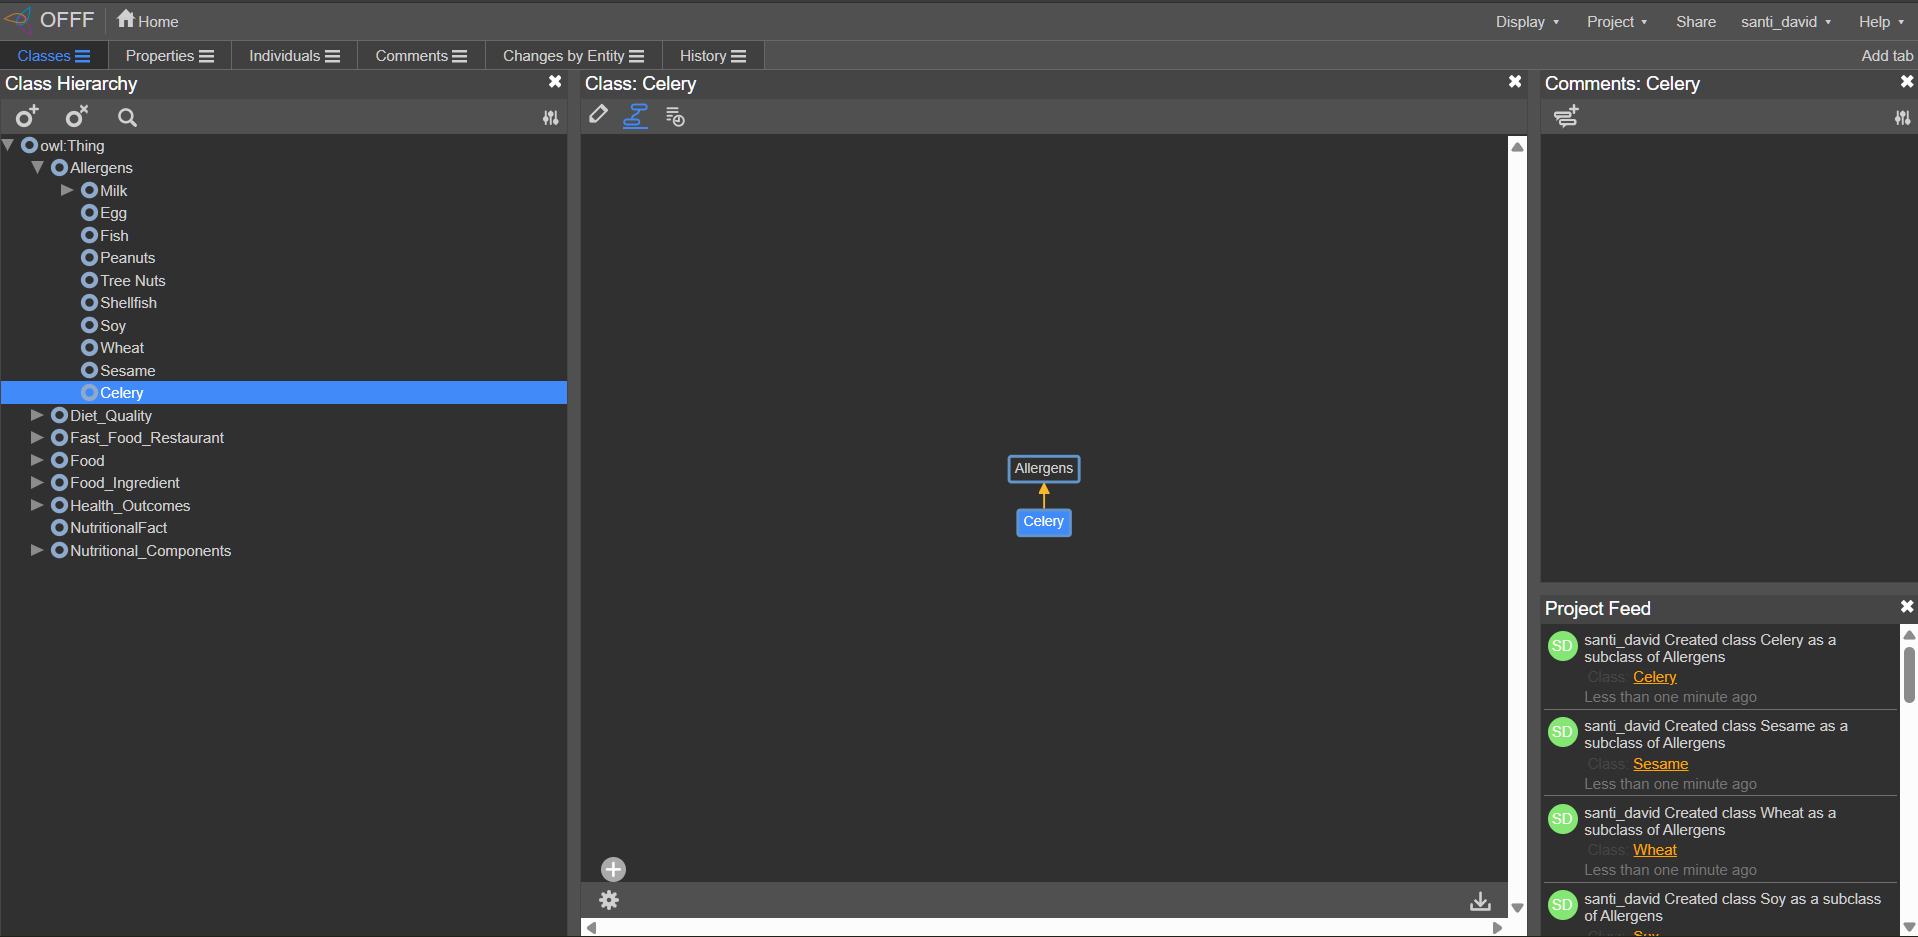
\includegraphics[width=0.8\textwidth]{screenshots/Allergens.png}
    \caption{Class hierarchy showing the 10 new Allergens subclasses. Username \texttt{santi\_david} is visible in the WebProtégé interface.}
    \label{fig:allergens_hierarchy}
\end{figure}

\subsubsection{Technical Explanation}

\begin{itemize}
    \item \textbf{Taxonomic relationship:} A \texttt{SubClassOf} relationship is established between each allergen and the \texttt{Allergens} class
    \item \textbf{Inheritance:} Each subclass inherits the properties and restrictions of the parent class
    \item \textbf{Reasoning:} A reasoner can infer that any instance of \texttt{Peanut} is also an instance of \texttt{Allergens}
    \item \textbf{Extensibility:} The structure allows adding new allergens in the future without modifying the base ontology
\end{itemize}

\subsection{Allergy Class in Health\_Outcomes}

\subsubsection{Objective}

Create a new \texttt{Allergy} class as a subclass of \texttt{Health\_Outcomes} and establish causal relationships between allergens and this new health condition.

\subsubsection{Creation Process}

\begin{enumerate}
    \item \textbf{Locate parent class:} Navigate to the \texttt{Health\_Outcomes} class
    \item \textbf{Create subclass:} Use ``Create subclass'' with the name \texttt{Allergy}
    \item \textbf{Define causal relationships:} Establish that \texttt{Allergy} is caused by each of the 10 allergens
\end{enumerate}

\subsubsection{\texttt{causedBy} Relationships}

Ten class axioms were established using the object property \texttt{causedBy}:

\begin{verbatim}
Allergy SubClassOf causedBy some Peanut
Allergy SubClassOf causedBy some TreeNuts
Allergy SubClassOf causedBy some Milk
Allergy SubClassOf causedBy some Egg
Allergy SubClassOf causedBy some Fish
Allergy SubClassOf causedBy some Shellfish
Allergy SubClassOf causedBy some Soy
Allergy SubClassOf causedBy some Wheat
Allergy SubClassOf causedBy some Sesame
Allergy SubClassOf causedBy some Celery
\end{verbatim}

\subsubsection{Graphical Evidence}

\begin{figure}[H]
    \centering
    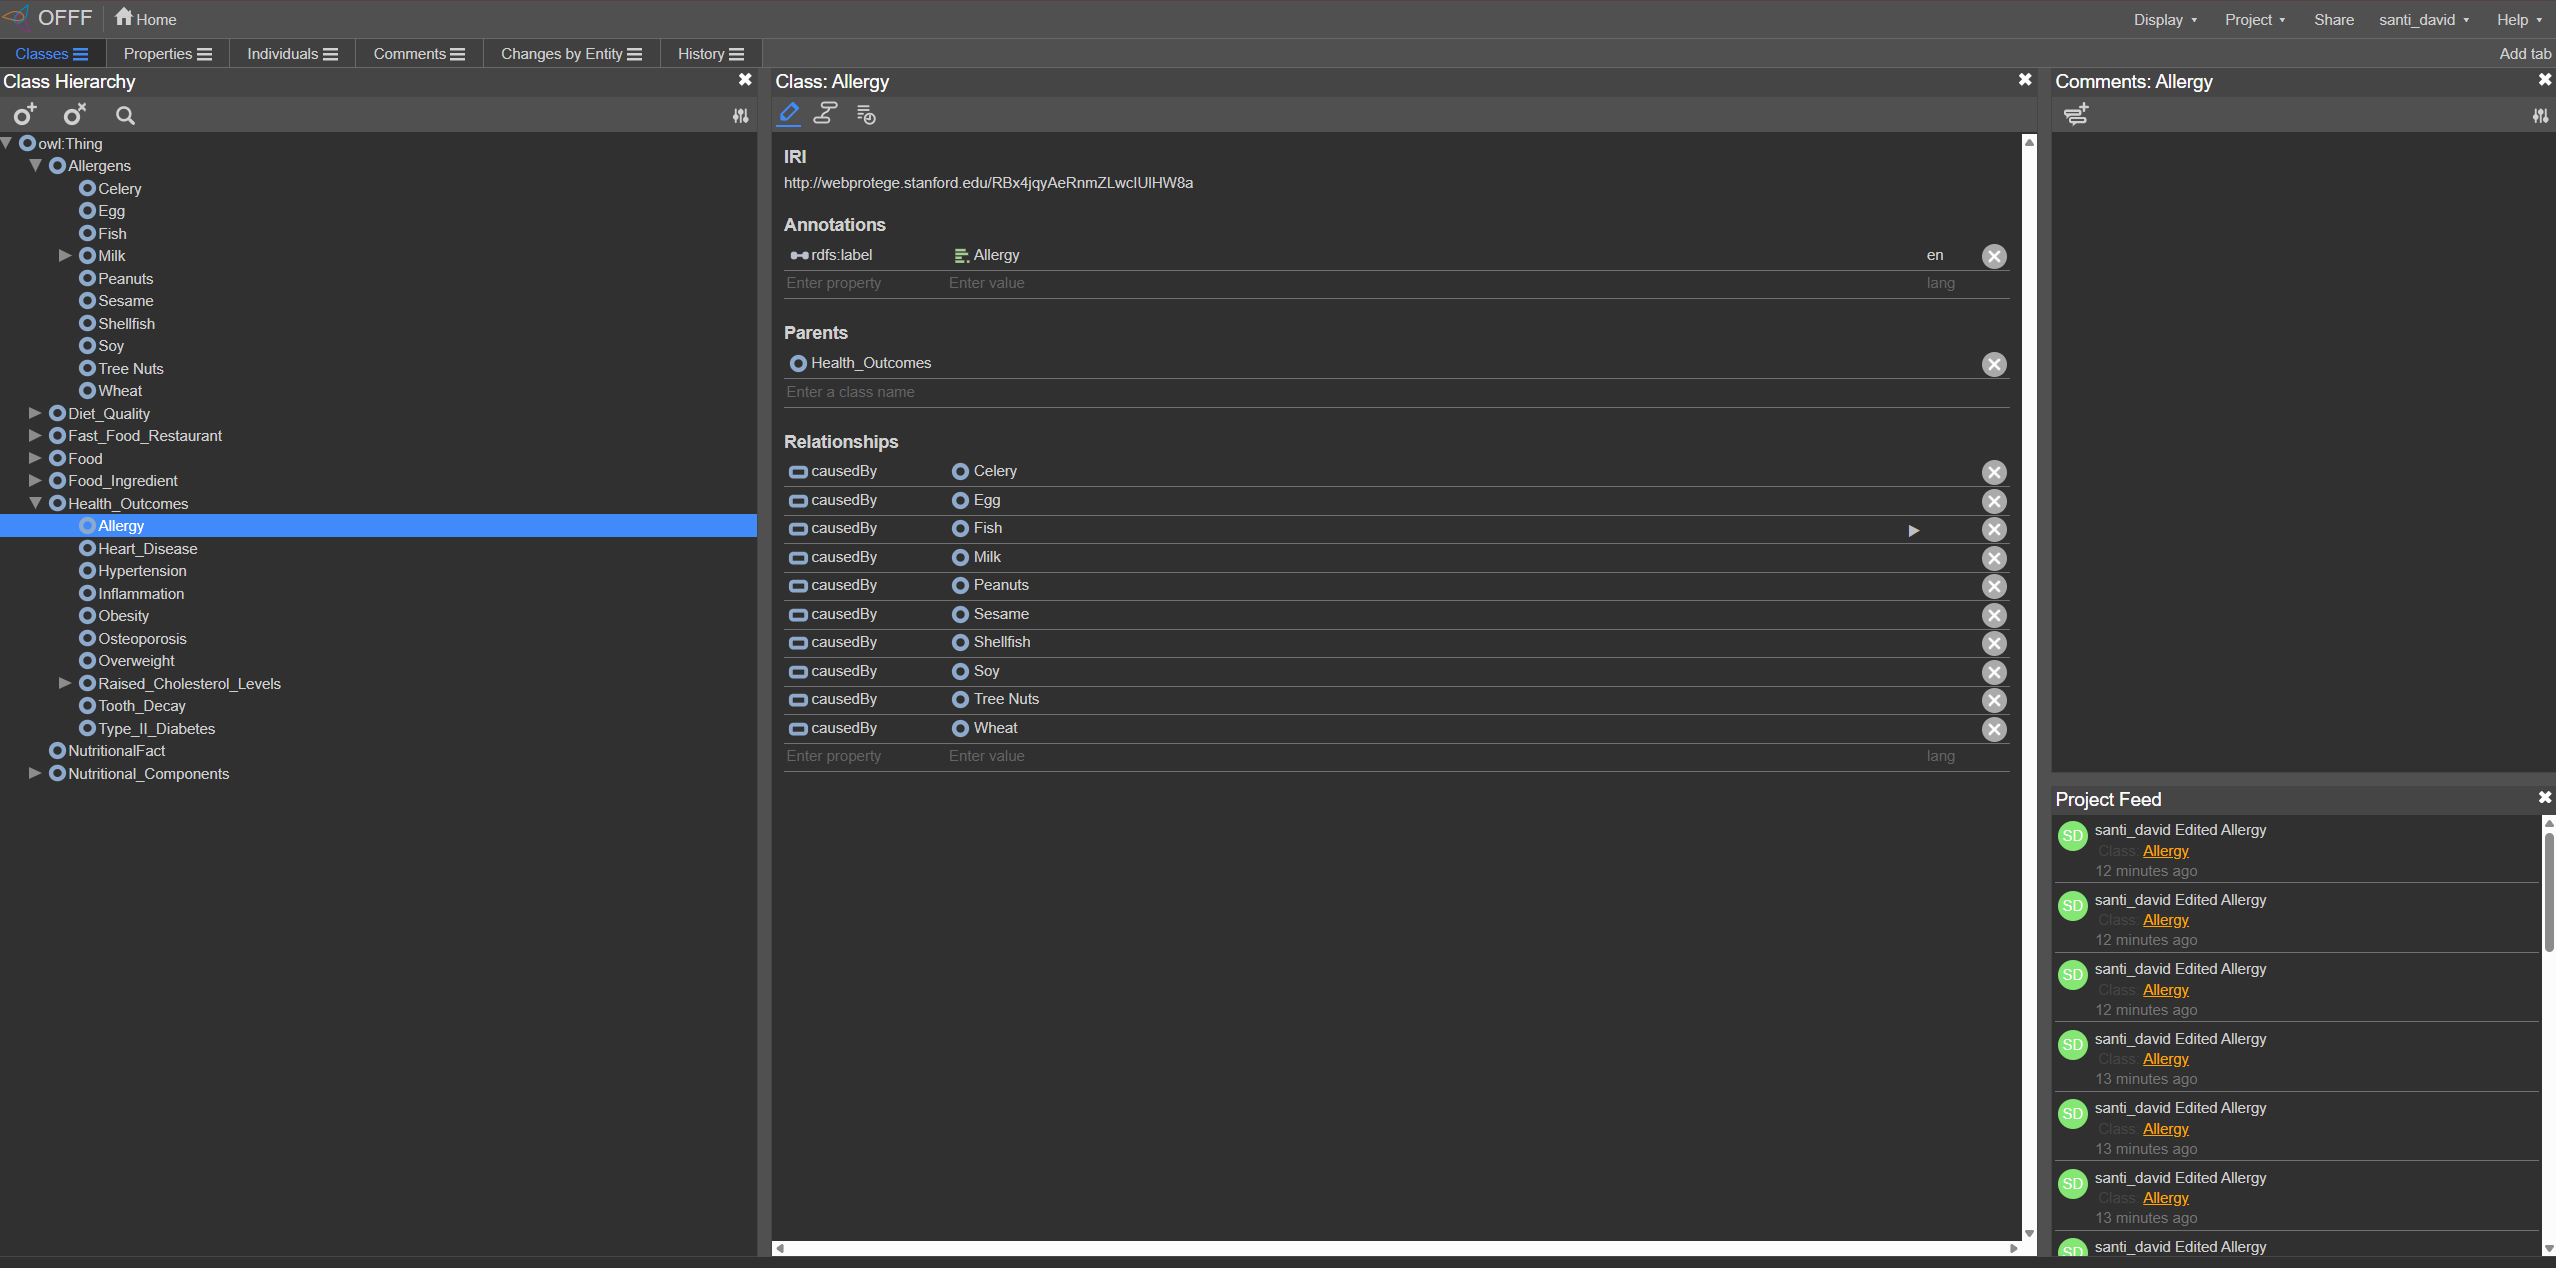
\includegraphics[width=0.8\textwidth]{screenshots/allergy.png}
    \caption{Allergy class created in Health\_Outcomes with its causal relationships. Visible username: \texttt{santi\_david}}
    \label{fig:allergy_class}
\end{figure}

\subsubsection{Technical Explanation}

\begin{itemize}
    \item \textbf{Object property:} \texttt{causedBy} is an existing object property in OFFF that relates \texttt{Health\_Outcomes} to \texttt{Diet\_Quality} or food components
    \item \textbf{Existential restriction (some):} Indicates that there exists at least one causal relationship
    \item \textbf{Semantics:} ``An allergy is a health outcome that can be caused by any of the defined allergens''
    \item \textbf{Reasoning:} A reasoner can infer that if a food contains \texttt{Peanut}, it can cause \texttt{Allergy}
\end{itemize}

\subsection{Inflammation Class in Health\_Outcomes}

\subsubsection{Objective}

Create the \texttt{Inflammation} class and establish that various chronic diseases are caused by inflammatory processes.

\subsubsection{Creation Process}

Similar to the previous process:
\begin{enumerate}
    \item Create \texttt{Inflammation} as a subclass of \texttt{Health\_Outcomes}
    \item Establish inverse causal relationships with 4 existing health conditions
\end{enumerate}

\subsubsection{Causal Relationships}

It was established that the following conditions are caused by inflammation:

\begin{enumerate}
    \item \texttt{Heart\_Disease}: Cardiovascular diseases
    \item \texttt{Hypertension}: Arterial hypertension
    \item \texttt{Obesity}: Obesity
    \item \texttt{Type\_II\_Diabetes}: Type 2 diabetes
\end{enumerate}

The established axioms were:

\begin{verbatim}
Heart_Disease SubClassOf causedBy some Inflammation
Hypertension SubClassOf causedBy some Inflammation
Obesity SubClassOf causedBy some Inflammation
Type_II_Diabetes SubClassOf causedBy some Inflammation
\end{verbatim}

\subsubsection{Graphical Evidence}

\begin{figure}[H]
    \centering
    \begin{subfigure}[b]{0.45\textwidth}
        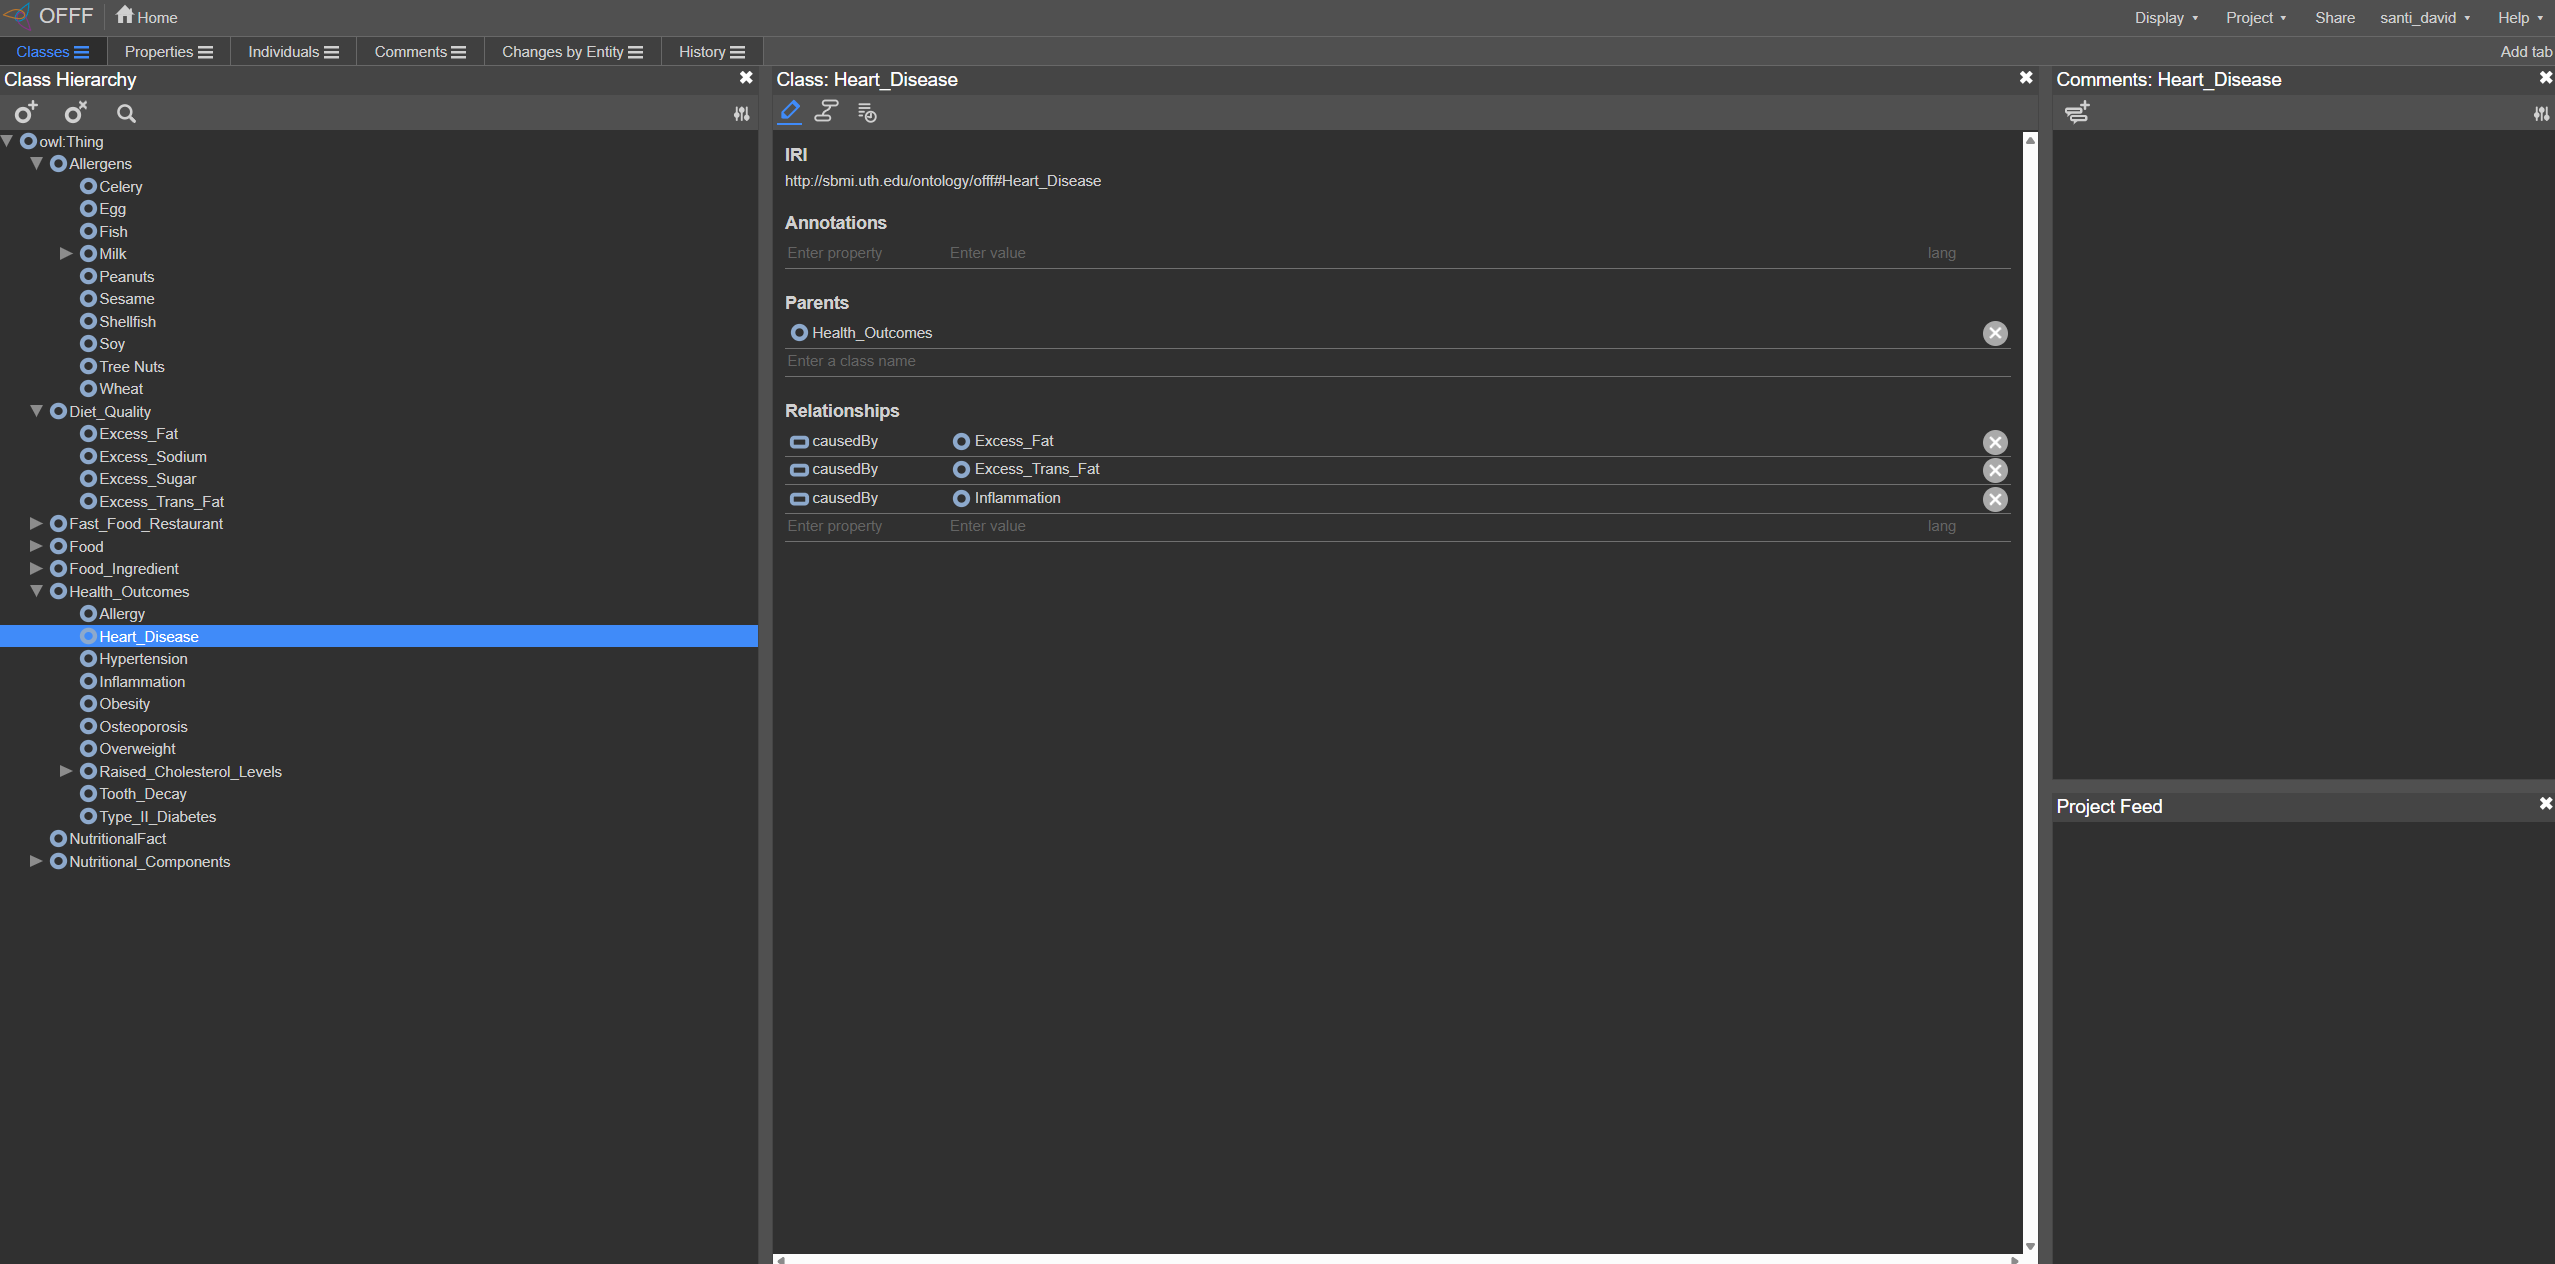
\includegraphics[width=\textwidth]{screenshots/inflammation_1.png}
        \caption{Relationship with Heart Disease}
    \end{subfigure}
    \hfill
    \begin{subfigure}[b]{0.45\textwidth}
        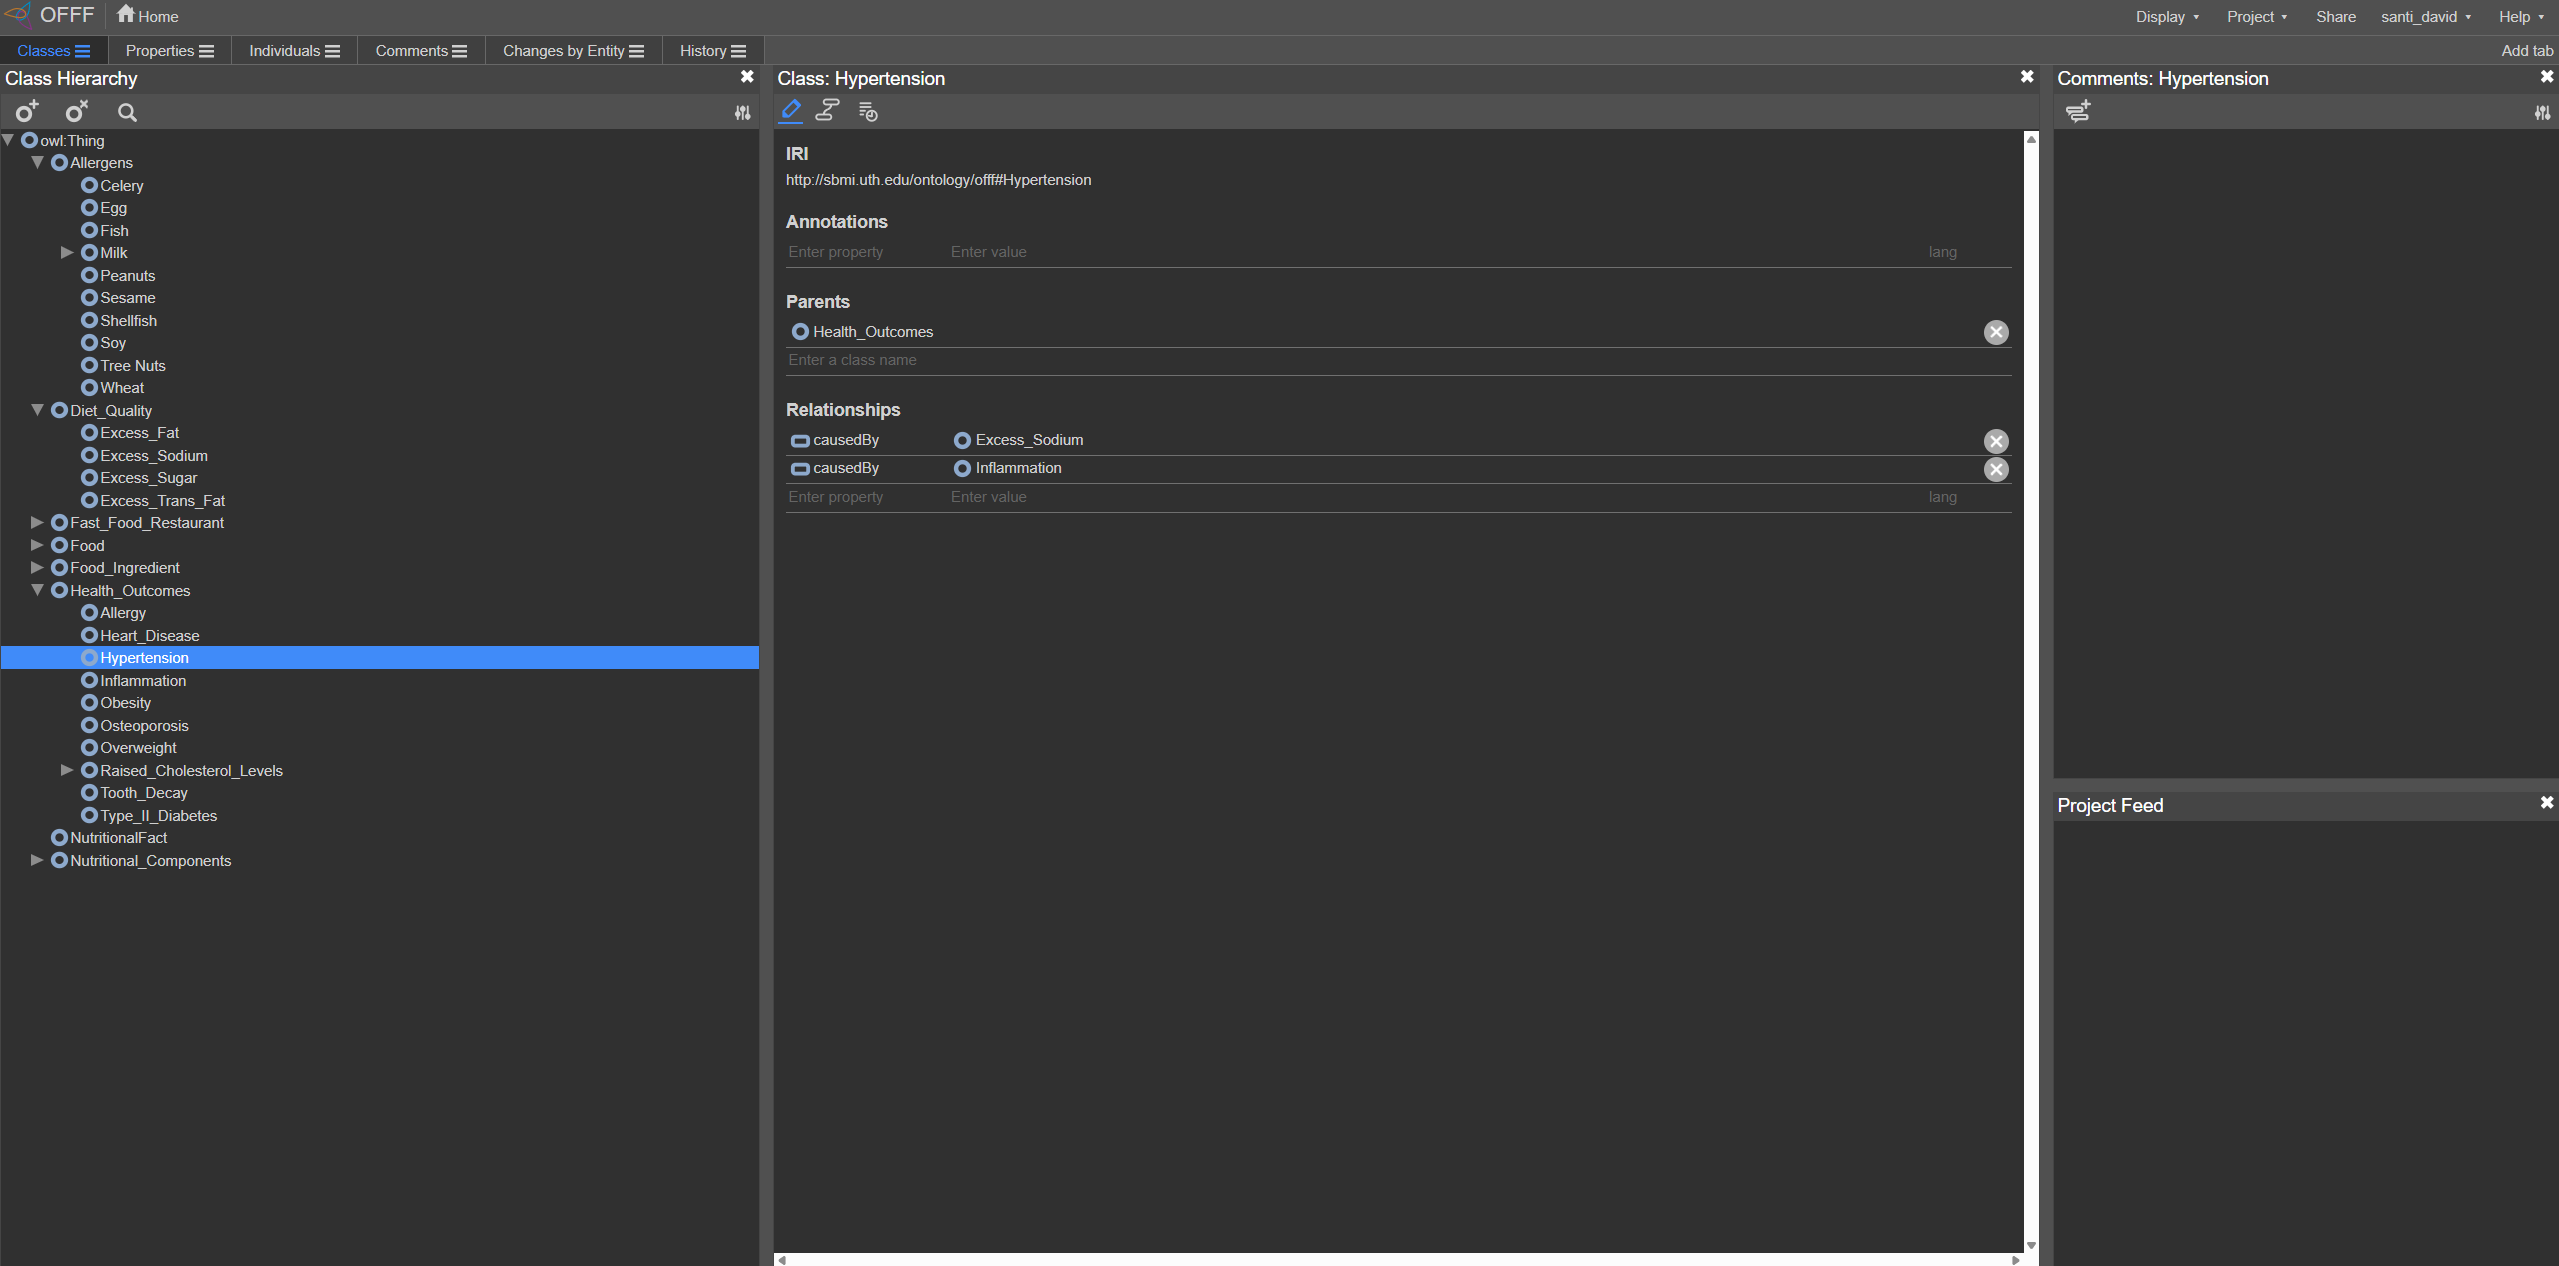
\includegraphics[width=\textwidth]{screenshots/inflammation_2.png}
        \caption{Relationship with Hypertension}
    \end{subfigure}
    
    \vspace{0.5cm}
    
    \begin{subfigure}[b]{0.45\textwidth}
        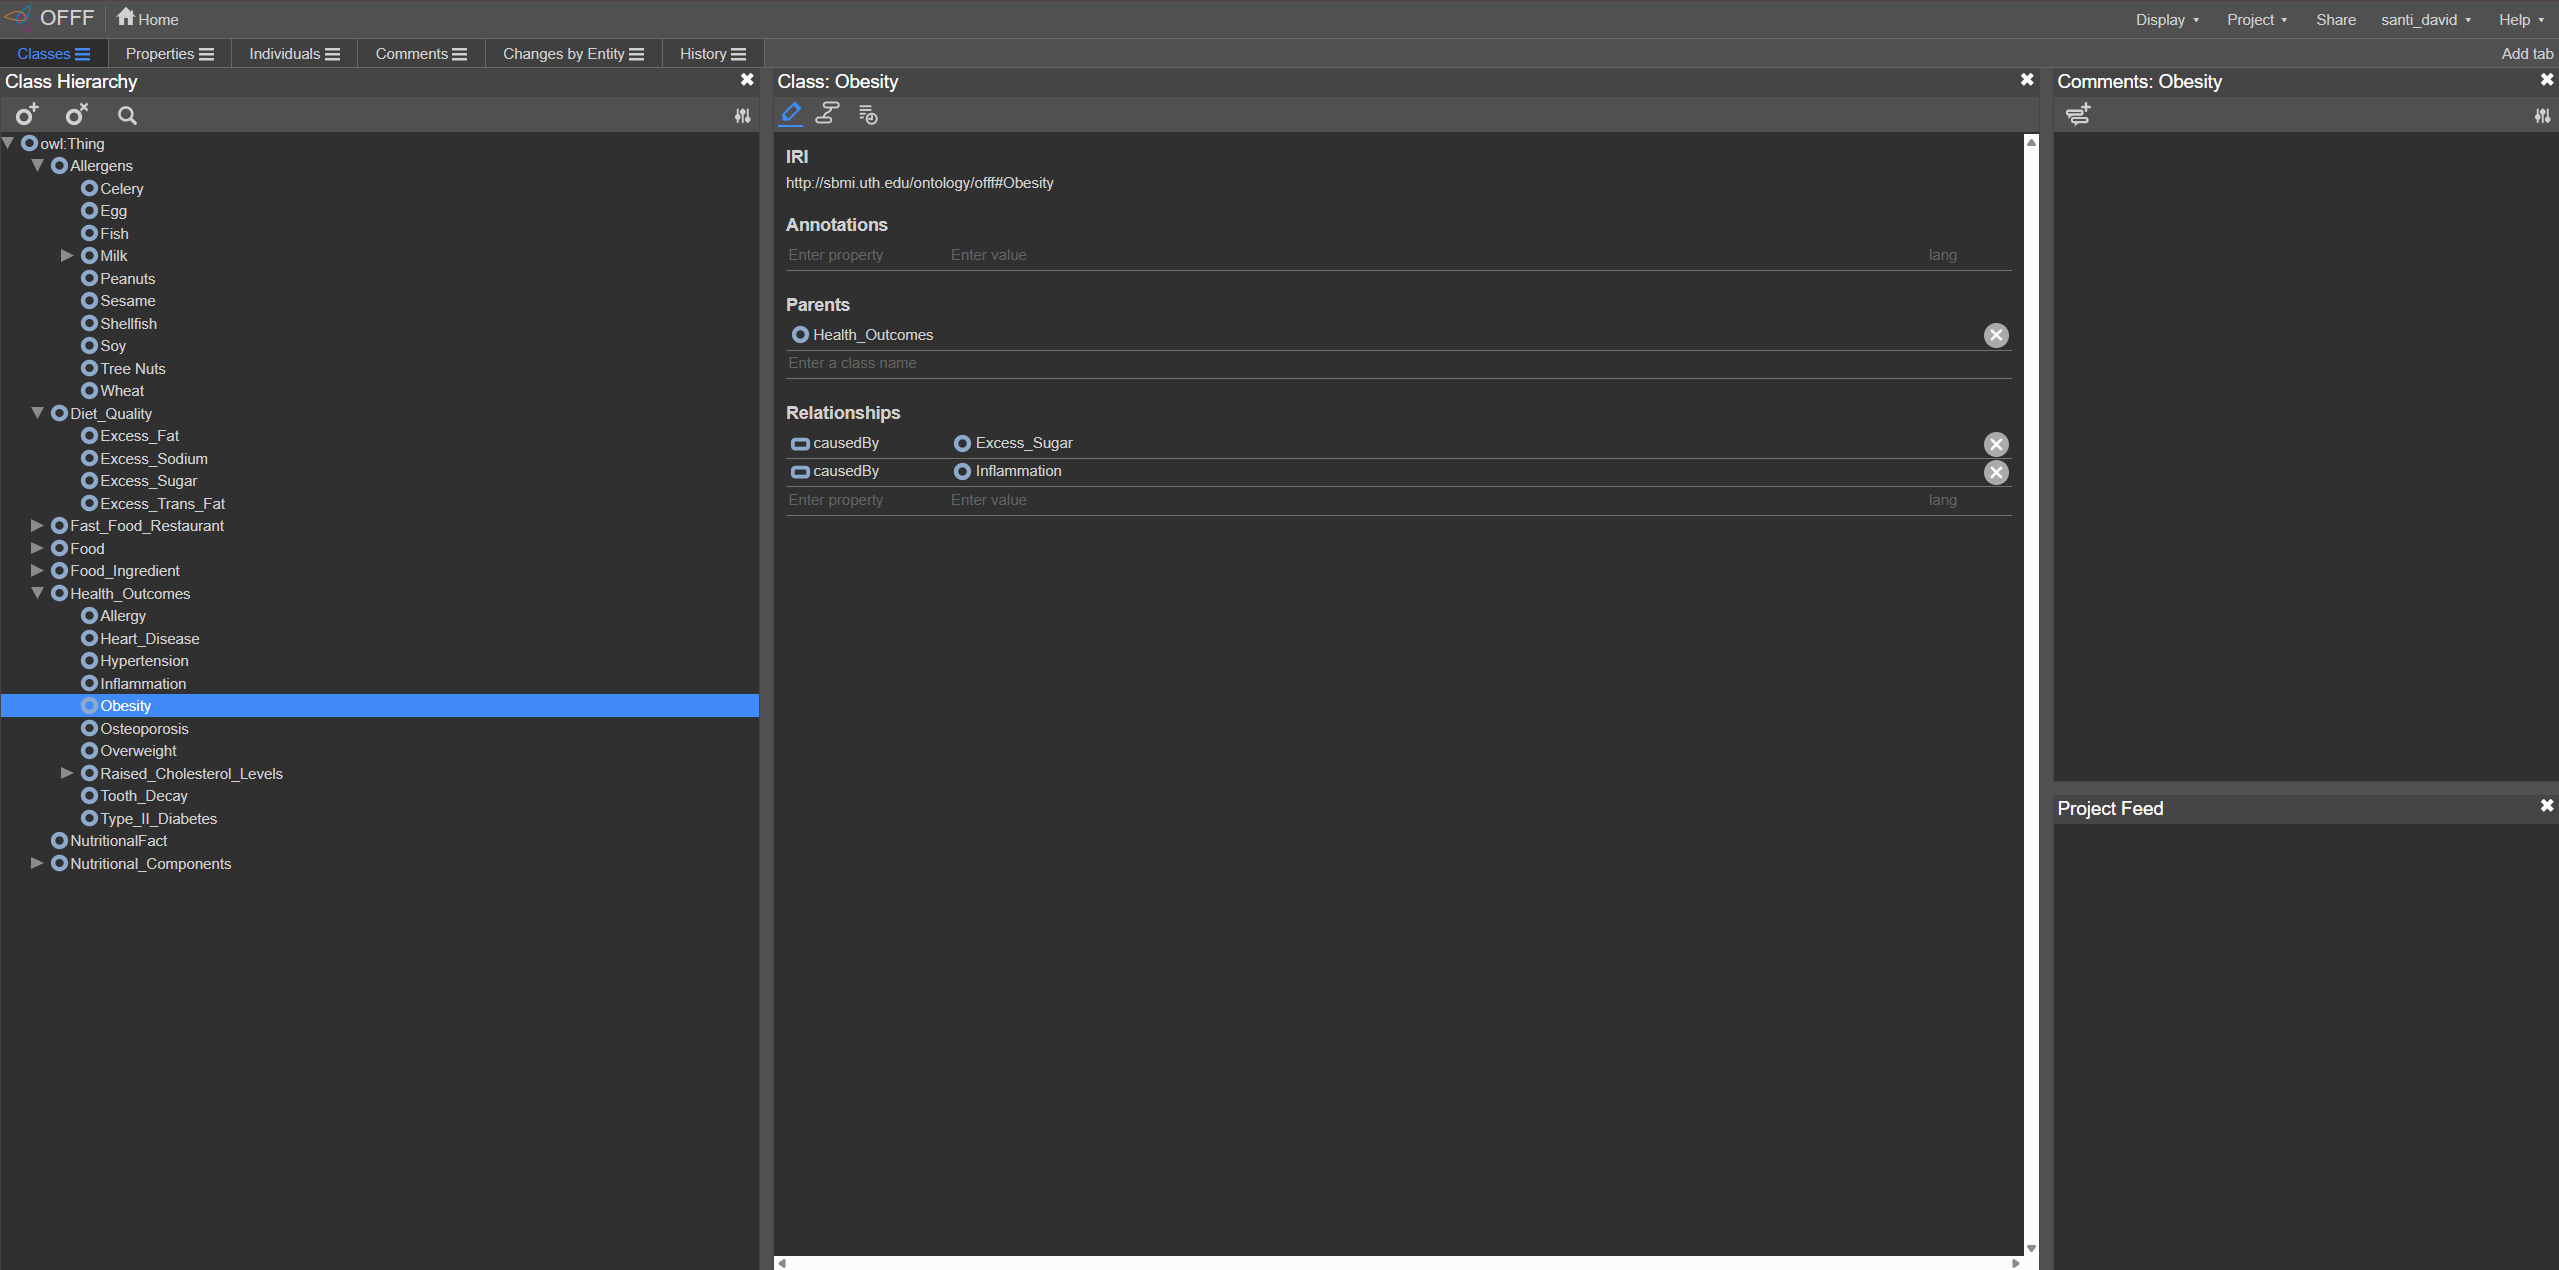
\includegraphics[width=\textwidth]{screenshots/inflammation_3.png}
        \caption{Relationship with Obesity}
    \end{subfigure}
    \hfill
    \begin{subfigure}[b]{0.45\textwidth}
        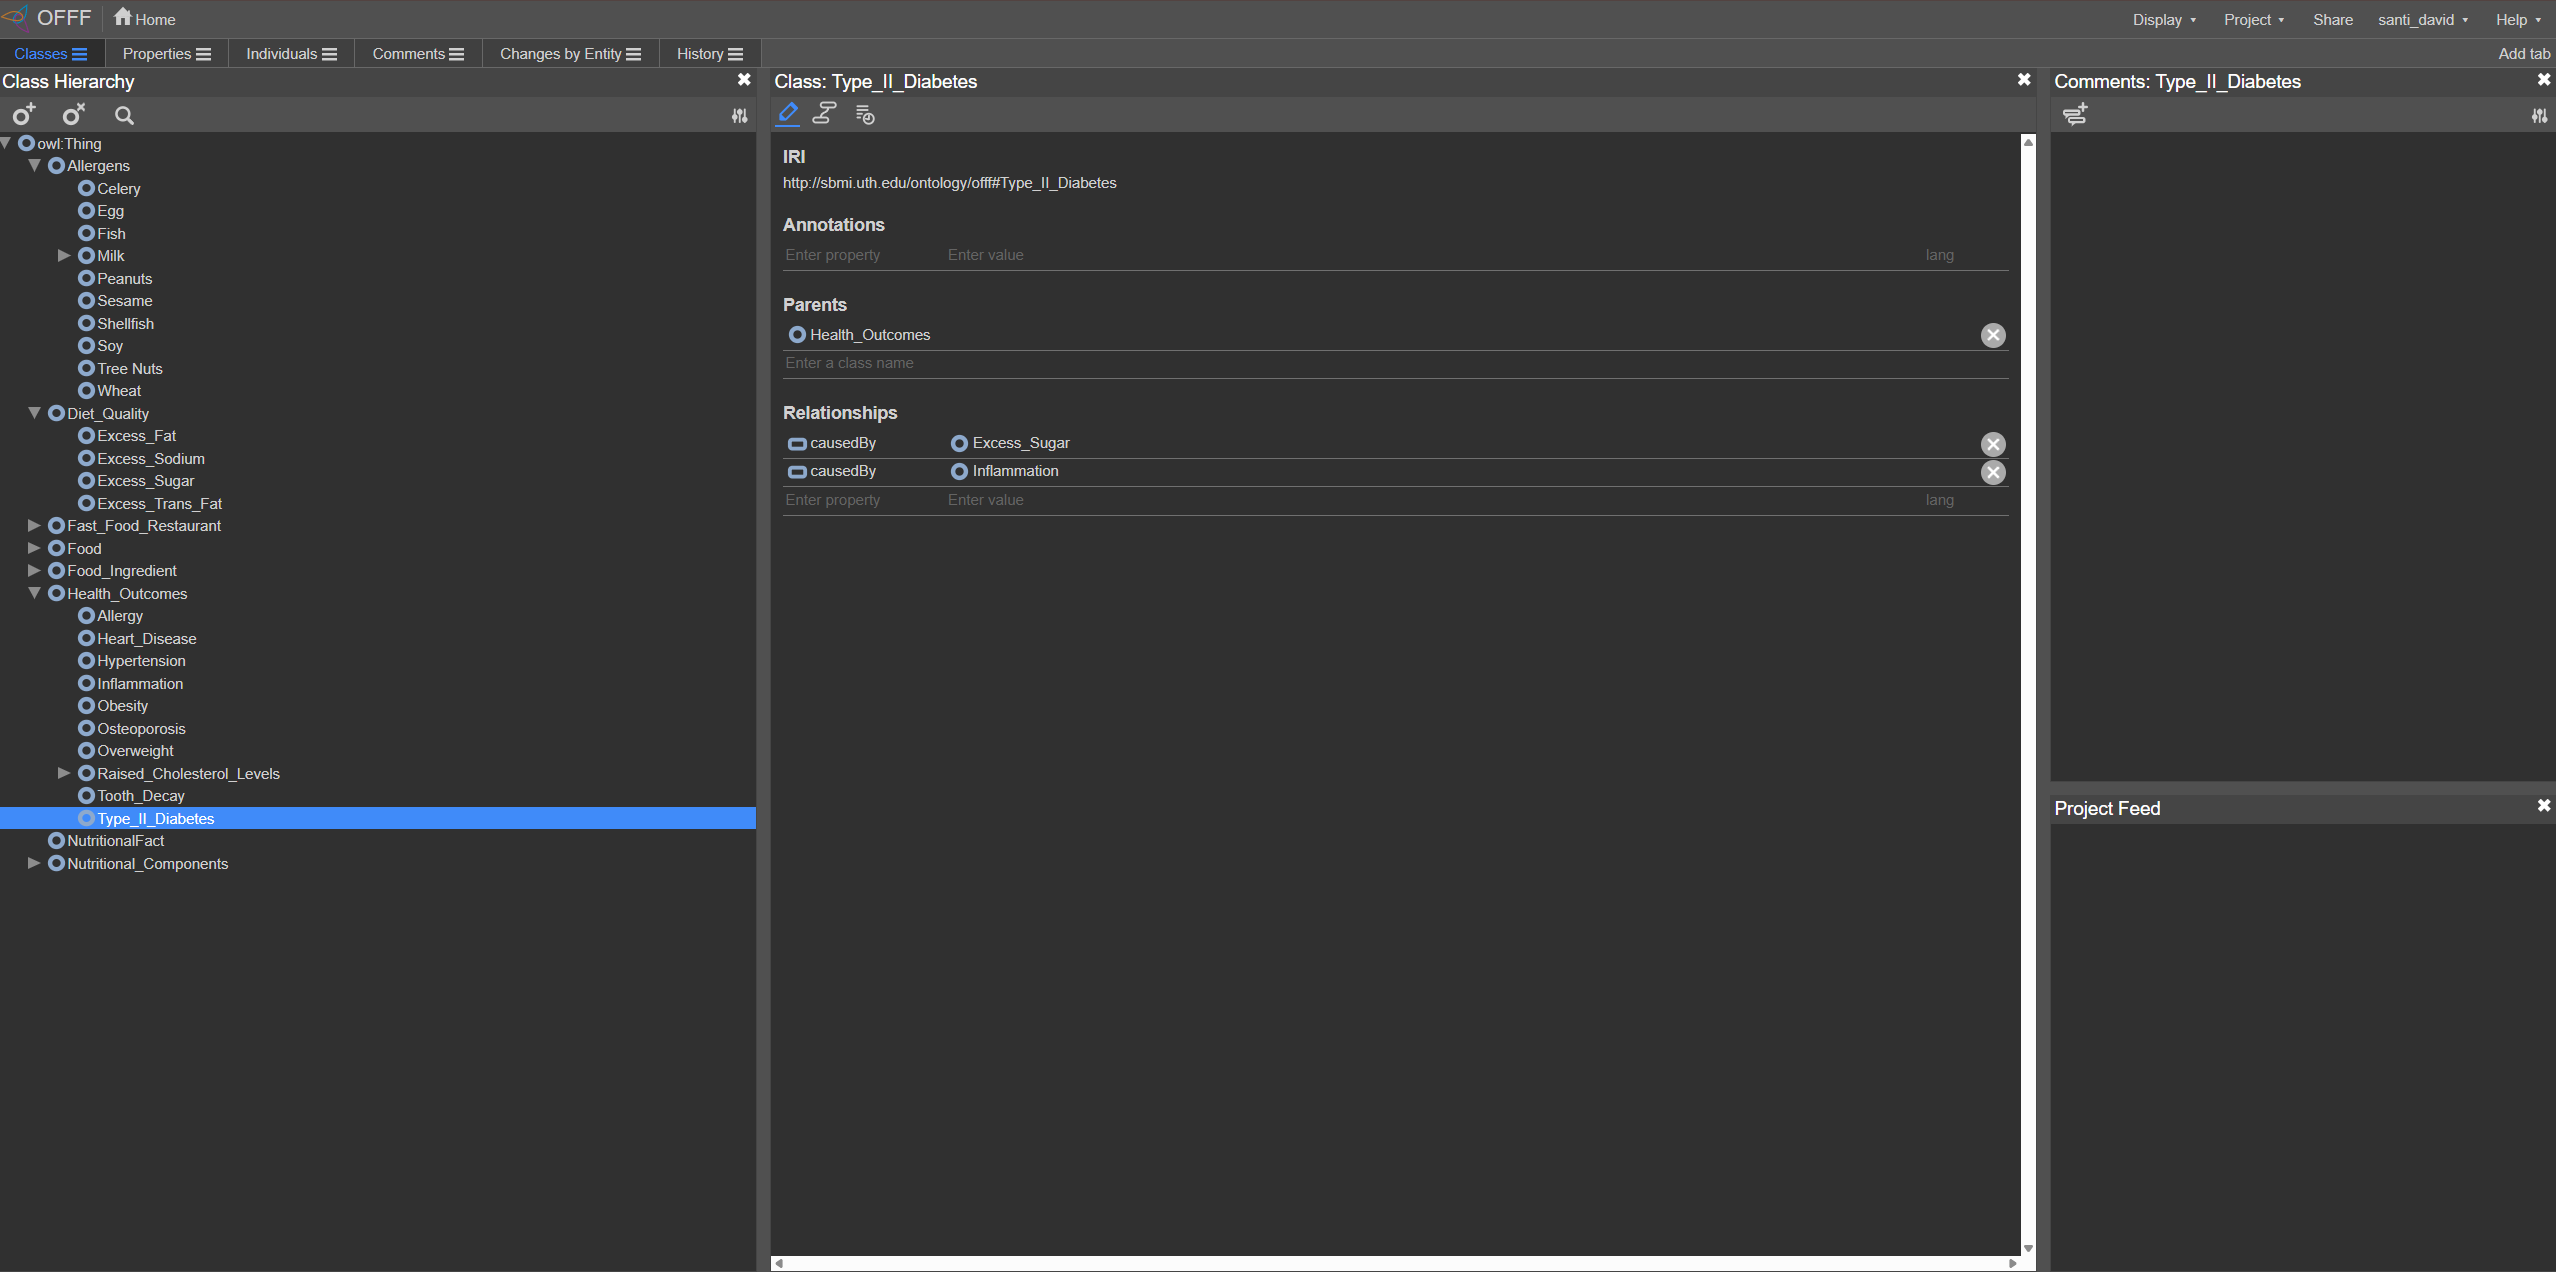
\includegraphics[width=\textwidth]{screenshots/inflammation_4.png}
        \caption{Relationship with Type II Diabetes}
    \end{subfigure}
    
    \caption{Inflammation class and its causal relationships with chronic diseases. Username \texttt{santi\_david} visible in all screenshots.}
    \label{fig:inflammation_relations}
\end{figure}

\subsubsection{Scientific Justification}

Chronic inflammation is an underlying factor in many modern diseases:

\begin{itemize}
    \item \textbf{Heart diseases:} Inflammation contributes to atherosclerosis
    \item \textbf{Hypertension:} Inflammatory processes affect endothelial function
    \item \textbf{Obesity:} Excess adipose tissue produces inflammatory cytokines
    \item \textbf{Type 2 diabetes:} Inflammation interferes with insulin signaling
\end{itemize}

\subsubsection{Technical Explanation}

\begin{itemize}
    \item \textbf{Relationship direction:} Established from diseases toward \texttt{Inflammation} using \texttt{causedBy}
    \item \textbf{Interpretation:} These diseases are results of chronic inflammatory processes
    \item \textbf{Causal chain:} Allows reasoning about chains: Diet → Inflammation → Disease
\end{itemize}

\subsection{Individual ``My fish sandwich''}

\subsubsection{Objective}

Create a concrete instance of a food product (\texttt{Fish\_Sandwich}) with specific properties related to allergens.

\subsubsection{Creation Process}

\begin{enumerate}
    \item \textbf{Locate class:} Find \texttt{Fish\_Sandwich} in the hierarchy (subclass of \texttt{Fast\_Food})
    \item \textbf{Create instance:} Go to the ``Individuals'' tab and create a new individual
    \item \textbf{Assign type:} Set \texttt{Fish\_Sandwich} as the class type
    \item \textbf{Add data properties:} Assign values to data properties
\end{enumerate}

\subsubsection{Assigned Data Properties}

\begin{enumerate}
    \item \textbf{containsGluten:} \texttt{true}
    \begin{itemize}
        \item Type: \texttt{xsd:boolean}
        \item Meaning: The sandwich contains gluten (from bread)
    \end{itemize}
    
    \item \textbf{hasAllergen:} \texttt{``Peanut Oil''}
    \begin{itemize}
        \item Type: \texttt{xsd:string}
        \item Meaning: Peanut oil was used in preparation
    \end{itemize}
\end{enumerate}

\subsubsection{Graphical Evidence}

\begin{figure}[H]
    \centering
    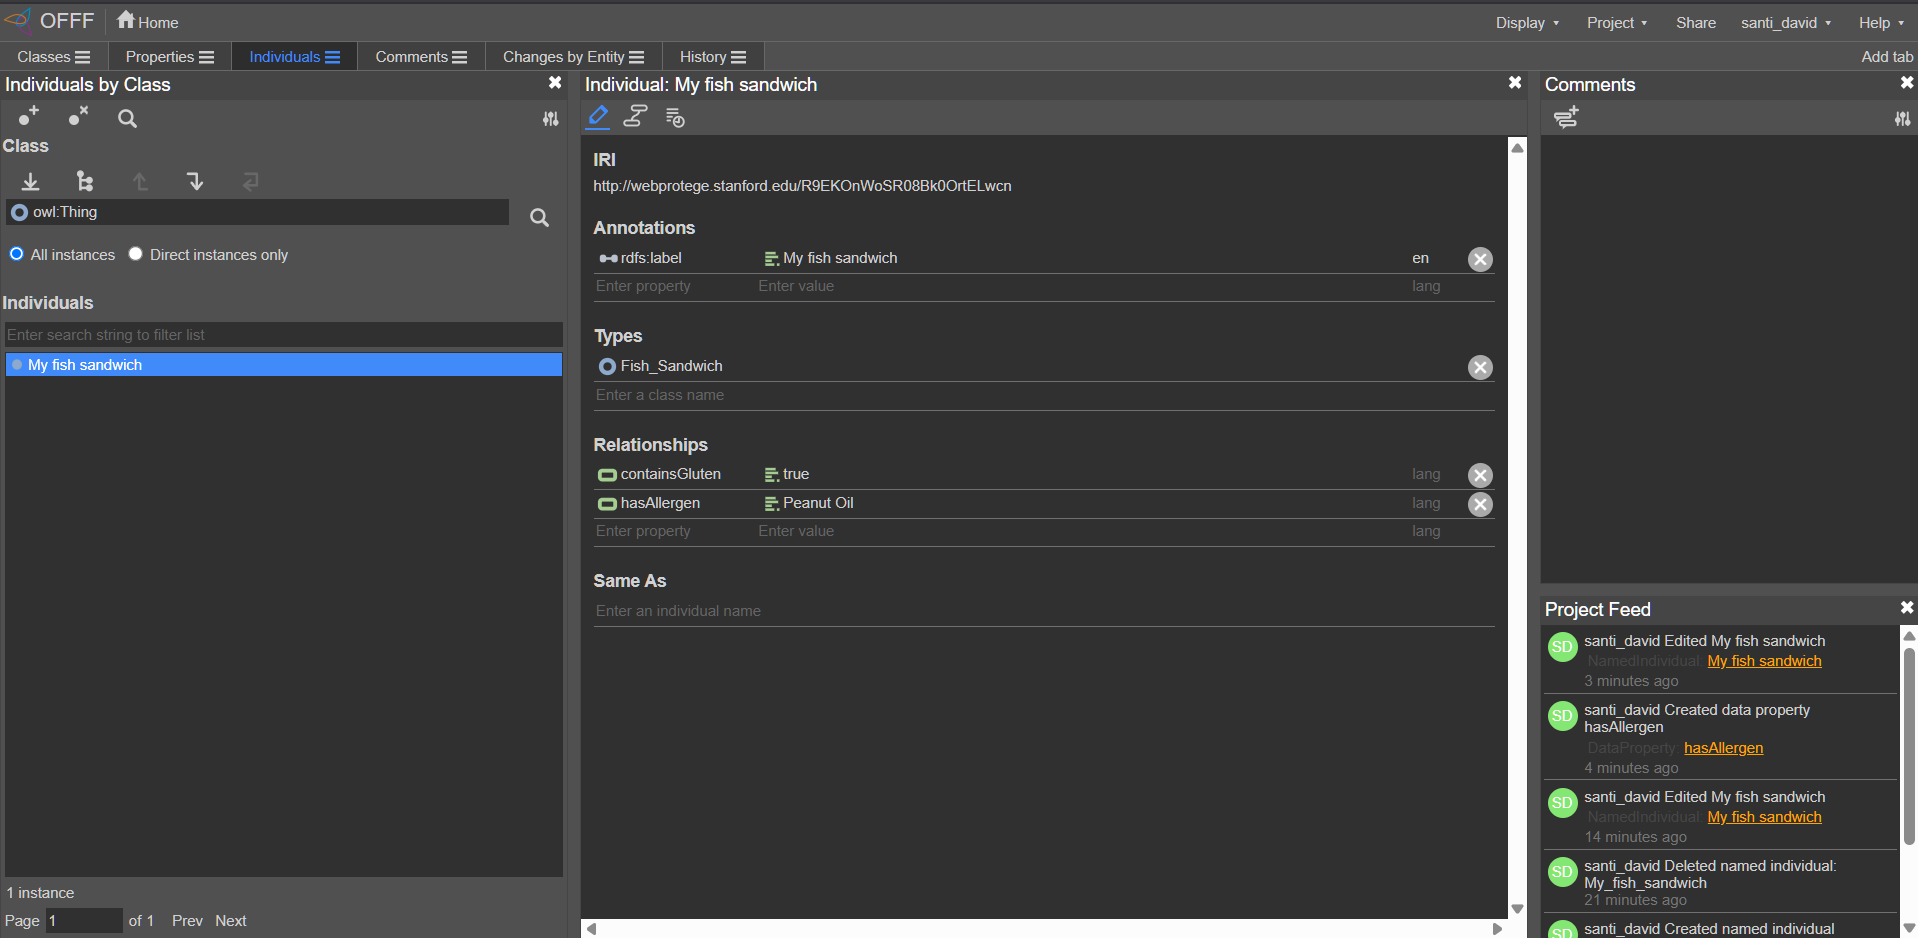
\includegraphics[width=0.8\textwidth]{screenshots/My fish sandwich.png}
    \caption{Individual ``My fish sandwich'' with its data properties. Username \texttt{santi\_david} visible.}
    \label{fig:my_fish_sandwich}
\end{figure}

\subsubsection{Technical Explanation}

\begin{itemize}
    \item \textbf{Instance vs Class:} This is a concrete individual, not a category
    \item \textbf{ABox vs TBox:} Instances are part of the ABox (data), while classes form the TBox (terminology)
    \item \textbf{Data properties:} Connect individuals with literal values (strings, numbers, booleans)
    \item \textbf{Inference:} A reasoner can infer that this sandwich may cause allergies in people sensitive to peanuts or gluten
    \item \textbf{Practical utility:} Allows labeling specific products with allergen information for recommendation systems
\end{itemize}

\subsubsection{Implications}

This individual exemplifies how ontologies can be used to:
\begin{itemize}
    \item Label products with allergen information
    \item Facilitate searches (``find gluten-free sandwiches'')
    \item Warn consumers about potential risks
    \item Comply with food labeling regulations
\end{itemize}

%==============================================================================
% SECTION 3: SPARQL QUERIES
%==============================================================================
\section{SPARQL Queries}

SPARQL (SPARQL Protocol and RDF Query Language) is the standard language for querying RDF data on the Semantic Web. This section presents three queries performed on DBpedia, the semantic version of Wikipedia.

\subsection{Query 1: Artists in DBpedia}

\subsubsection{Objective}

Obtain 10 artist names whose names begin with ``Mado'' using the DBpedia SPARQL endpoint.

\subsubsection{Endpoint}

\begin{itemize}
    \item \textbf{URL:} \url{https://dbpedia.org/sparql/}
    \item \textbf{Endpoint URI:} \texttt{http://dbpedia.org}
\end{itemize}

\subsubsection{SPARQL Query}

\begin{lstlisting}[language=SPARQL, caption={Query 1: Artists starting with ``Mado''}]
PREFIX dbo: <http://dbpedia.org/ontology/>
PREFIX rdfs: <http://www.w3.org/2000/01/rdf-schema#>

SELECT DISTINCT ?artist ?name
WHERE {
  ?artist a dbo:Artist .
  ?artist rdfs:label ?name .
  FILTER (lang(?name) = 'en')
  FILTER (STRSTARTS(?name, "Mado"))
}
LIMIT 10
\end{lstlisting}

\subsubsection{Detailed Explanation}

\begin{enumerate}
    \item \textbf{PREFIX declarations:}
    \begin{itemize}
        \item \texttt{dbo:} DBpedia Ontology (\texttt{http://dbpedia.org/ontology/})
        \item \texttt{rdfs:} RDF Schema (\texttt{http://www.w3.org/2000/01/rdf-schema\#})
    \end{itemize}
    
    \item \textbf{SELECT DISTINCT:} Selects unique values of variables \texttt{?artist} and \texttt{?name}, avoiding duplicates
    
    \item \textbf{Triple patterns:}
    \begin{itemize}
        \item \texttt{?artist a dbo:Artist}: Filters only entities of type \texttt{Artist}
        \item \texttt{?artist rdfs:label ?name}: Gets the label (name) of the artist
    \end{itemize}
    
    \item \textbf{FILTER (lang(?name) = 'en'):} Filters only labels in English language
    
    \item \textbf{FILTER (STRSTARTS(?name, ``Mado'')):} String function that verifies if the name starts with ``Mado''
    
    \item \textbf{LIMIT 10:} Limits results to 10 artists
\end{enumerate}

\subsubsection{Results}

\begin{figure}[H]
    \centering
    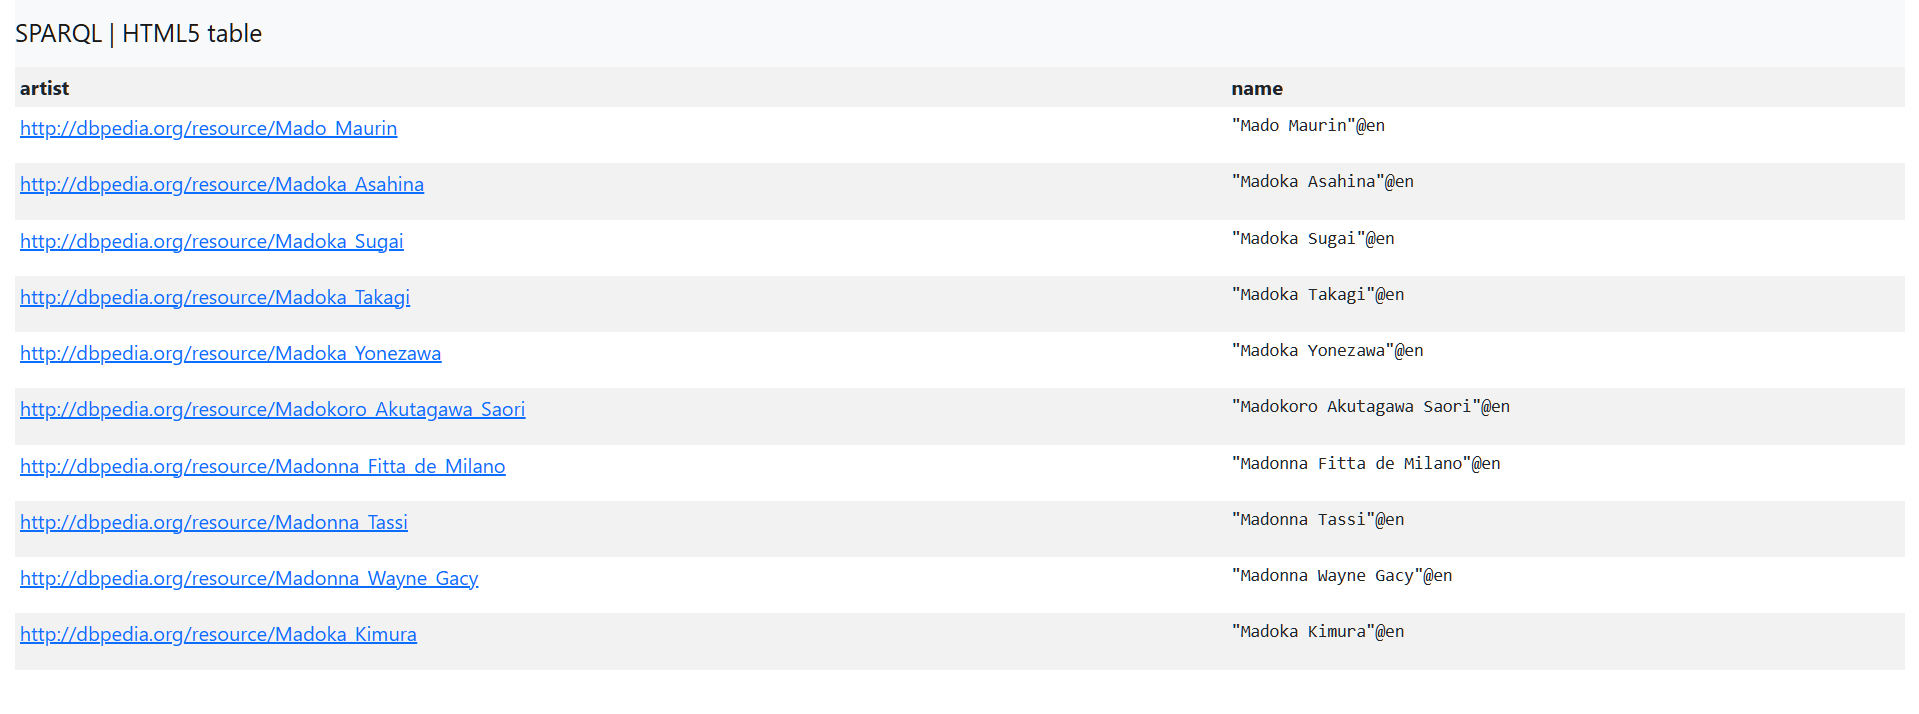
\includegraphics[width=\textwidth]{screenshots/Query1.png}
    \caption{Results of Query 1 executed on DBpedia SPARQL Endpoint}
    \label{fig:query1_results}
\end{figure}

\begin{table}[H]
    \centering
    \caption{Artists starting with ``Mado''}
    \label{tab:query1_results}
    \begin{tabular}{|l|l|}
        \hline
        \textbf{Artist URI} & \textbf{Name} \\
        \hline
        \url{http://dbpedia.org/resource/Mado_Maurin} & Mado Maurin \\
        \url{http://dbpedia.org/resource/Madoka_Asahina} & Madoka Asahina \\
        \url{http://dbpedia.org/resource/Madoka_Sugai} & Madoka Sugai \\
        \url{http://dbpedia.org/resource/Madoka_Takagi} & Madoka Takagi \\
        \url{http://dbpedia.org/resource/Madoka_Yonezawa} & Madoka Yonezawa \\
        \url{http://dbpedia.org/resource/Madokoro_Akutagawa_Saori} & Madokoro Akutagawa Saori \\
        \url{http://dbpedia.org/resource/Madonna_Fitta_de_Milano} & Madonna Fitta de Milano \\
        \url{http://dbpedia.org/resource/Madonna_Tassi} & Madonna Tassi \\
        \url{http://dbpedia.org/resource/Madonna_Wayne_Gacy} & Madonna Wayne Gacy \\
        \url{http://dbpedia.org/resource/Madoka_Kimura} & Madoka Kimura \\
        \hline
    \end{tabular}
\end{table}


\subsubsection{Results Analysis}

The results show various artists whose names begin with ``Mado''. The query demonstrates:
\begin{itemize}
    \item Text pattern filtering capability in SPARQL
    \item Use of string functions (\texttt{STRSTARTS})
    \item Language filtering in multilingual data
    \item Access to DBpedia's structured ontology
\end{itemize}

\subsection{Query 2: Persons by Height}

\subsubsection{Objective}

Obtain the first 10 persons with height between 1.8 and 2.3 meters, born after 1980, ordered by birth date.

\subsubsection{Endpoint}

\begin{itemize}
    \item \textbf{URL:} \url{https://dbpedia.org/snorql/}
\end{itemize}

\subsubsection{SPARQL Query}

\begin{lstlisting}[language=SPARQL, caption={Query 2: Persons by height and birth date}]
PREFIX dbo: <http://dbpedia.org/ontology/>
PREFIX rdfs: <http://www.w3.org/2000/01/rdf-schema#>

SELECT DISTINCT ?person ?name ?height ?birthDate
WHERE {
  ?person a dbo:Person .
  ?person rdfs:label ?name .
  ?person dbo:height ?height .
  ?person dbo:birthDate ?birthDate .
  
  FILTER (lang(?name) = 'en')
  FILTER (?height >= 1.8 && ?height <= 2.3)
  FILTER (YEAR(?birthDate) > 1980)
}
ORDER BY ?birthDate
LIMIT 10
\end{lstlisting}

\subsubsection{Detailed Explanation}

\begin{enumerate}
    \item \textbf{Selected variables:} person, name, height, and birth date
    
    \item \textbf{Triple patterns:}
    \begin{itemize}
        \item \texttt{?person a dbo:Person}: Filters entities of type Person
        \item \texttt{?person dbo:height ?height}: Gets the height property
        \item \texttt{?person dbo:birthDate ?birthDate}: Gets birth date
    \end{itemize}
    
    \item \textbf{FILTER (?height >= 1.8 \&\& ?height <= 2.3):} 
    \begin{itemize}
        \item Logical AND operators (\texttt{\&\&})
        \item Filters heights in the range [1.8m, 2.3m]
        \item Heights in DBpedia are in meters
    \end{itemize}
    
    \item \textbf{FILTER (YEAR(?birthDate) > 1980):}
    \begin{itemize}
        \item \texttt{YEAR()} function extracts the year from a date
        \item Filters persons born after 1980
    \end{itemize}
    
    \item \textbf{ORDER BY ?birthDate:} 
    \begin{itemize}
        \item Orders results by birth date
        \item Default is ascending (oldest first)
    \end{itemize}
    
    \item \textbf{LIMIT 10:} First 10 persons meeting the criteria
\end{enumerate}

\subsubsection{Results}

\begin{figure}[H]
    \centering
    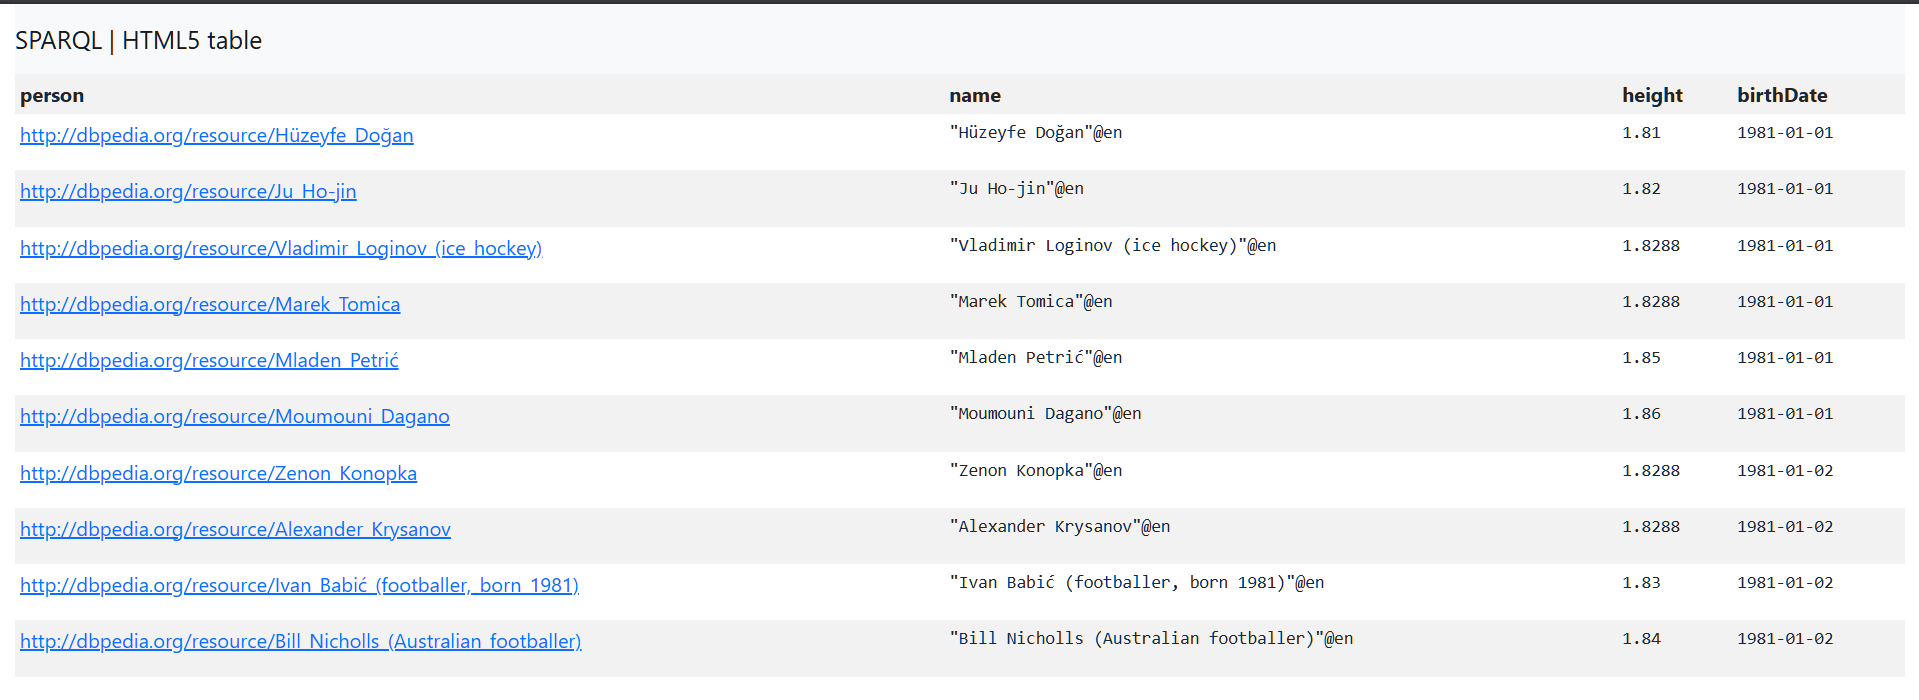
\includegraphics[width=\textwidth]{screenshots/Qiery2.png}
    \caption{Results of Query 2 executed on DBpedia Snorql}
    \label{fig:query2_results}
\end{figure}

\begin{table}[H]
    \centering
    \caption{Persons by height (1.8–2.3 m) born after 1980}
    \label{tab:query2_results}
    \resizebox{\linewidth}{!}{%
    \begin{tabular}{|l|l|c|c|}
        \hline
        \textbf{Person URI} & \textbf{Name} & \textbf{Height (m)} & \textbf{Birth Date} \\
        \hline
        \url{http://dbpedia.org/resource/Hüzeyfe_Doğan} & Hüzeyfe Doğan & 1.81 & 1981-01-01 \\
        \url{http://dbpedia.org/resource/Ju_Ho-jin} & Ju Ho-jin & 1.82 & 1981-01-01 \\
        \url{http://dbpedia.org/resource/Vladimir_Loginov_(ice_hockey)} & Vladimir Loginov (ice hockey) & 1.8288 & 1981-01-01 \\
        \url{http://dbpedia.org/resource/Marek_Tomica} & Marek Tomica & 1.8288 & 1981-01-01 \\
        \url{http://dbpedia.org/resource/Mladen_Petrić} & Mladen Petrić & 1.85 & 1981-01-01 \\
        \url{http://dbpedia.org/resource/Moumouni_Dagano} & Moumouni Dagano & 1.86 & 1981-01-01 \\
        \url{http://dbpedia.org/resource/Zenon_Konopka} & Zenon Konopka & 1.8288 & 1981-01-02 \\
        \url{http://dbpedia.org/resource/Alexander_Krysanov} & Alexander Krysanov & 1.8288 & 1981-01-02 \\
        \url{http://dbpedia.org/resource/Ivan_Babić_(footballer,_born_1981)} & Ivan Babić (footballer, born 1981) & 1.83 & 1981-01-02 \\
        \url{http://dbpedia.org/resource/Bill_Nicholls_(Australian_footballer)} & Bill Nicholls (Australian footballer) & 1.84 & 1981-01-02 \\
        \hline
    \end{tabular}
    } % end resizebox
\end{table}


\subsubsection{Results Analysis}

This query demonstrates:
\begin{itemize}
    \item \textbf{Numeric filters:} Value ranges for numeric properties
    \item \textbf{Date functions:} Extraction of temporal components
    \item \textbf{Ordering:} Results ordered chronologically
    \item \textbf{Complex queries:} Combination of multiple criteria
\end{itemize}

The results show relatively tall persons from the post-1980 generation, likely athletes or models.

\subsection{Query 3: Persons by Height/Weight and Clubs}

\subsubsection{Objective}

Obtain persons with height $\geq$ 2.10m OR weight $\geq$ 95kg, showing the number of associated clubs, grouped by person, ordered by number of clubs (ascending), limited to 7 results.

\subsubsection{Endpoint}

\begin{itemize}
    \item \textbf{URL:} \url{https://dbpedia.org/snorql/}
\end{itemize}

\subsubsection{SPARQL Query}

\begin{lstlisting}[language=SPARQL, caption={Query 3: Persons by height/weight and number of clubs}]
PREFIX dbo: <http://dbpedia.org/ontology/>
PREFIX rdfs: <http://www.w3.org/2000/01/rdf-schema#>

SELECT ?person ?name (COUNT(?club) as ?numberOfClubs)
WHERE {
  ?person a dbo:Person .
  ?person rdfs:label ?name .
  OPTIONAL { ?person dbo:team ?club . }
  
  {
    { ?person dbo:height ?height . FILTER (?height >= 2.10) }
    UNION
    { ?person dbo:weight ?weight . FILTER (?weight >= 95000) }
  }
  
  FILTER (lang(?name) = 'en')
}
GROUP BY ?person ?name
ORDER BY ASC(?numberOfClubs)
LIMIT 7
\end{lstlisting}

\subsubsection{Detailed Explanation}

\begin{enumerate}
    \item \textbf{SELECT with aggregation:}
    \begin{itemize}
        \item \texttt{COUNT(?club) as ?numberOfClubs}: Counts the number of clubs per person
        \item Aggregate function creates a new variable
    \end{itemize}
    
    \item \textbf{OPTIONAL \{ ?person dbo:team ?club . \}:}
    \begin{itemize}
        \item Optional pattern: doesn't discard persons without clubs
        \item Allows including persons with 0 clubs
    \end{itemize}
    
    \item \textbf{UNION between height and weight:}
    \begin{itemize}
        \item Logical OR operator: meet ANY of the conditions
        \item First branch: height $\geq$ 2.10 meters
        \item Second branch: weight $\geq$ 95000 grams (95 kg)
        \item Note: DBpedia stores weights in grams
    \end{itemize}
    
    \item \textbf{GROUP BY ?person ?name:}
    \begin{itemize}
        \item Groups results by person
        \item Necessary for aggregation functions (COUNT)
        \item Allows counting clubs per person
    \end{itemize}
    
    \item \textbf{ORDER BY ASC(?numberOfClubs):}
    \begin{itemize}
        \item Orders by number of clubs ascending
        \item \texttt{ASC}: ascending order (explicit)
        \item Persons with fewer clubs appear first
    \end{itemize}
    
    \item \textbf{LIMIT 7:} First 7 persons according to the ordering criterion
\end{enumerate}

\subsubsection{Results}

\begin{figure}[H]
    \centering
    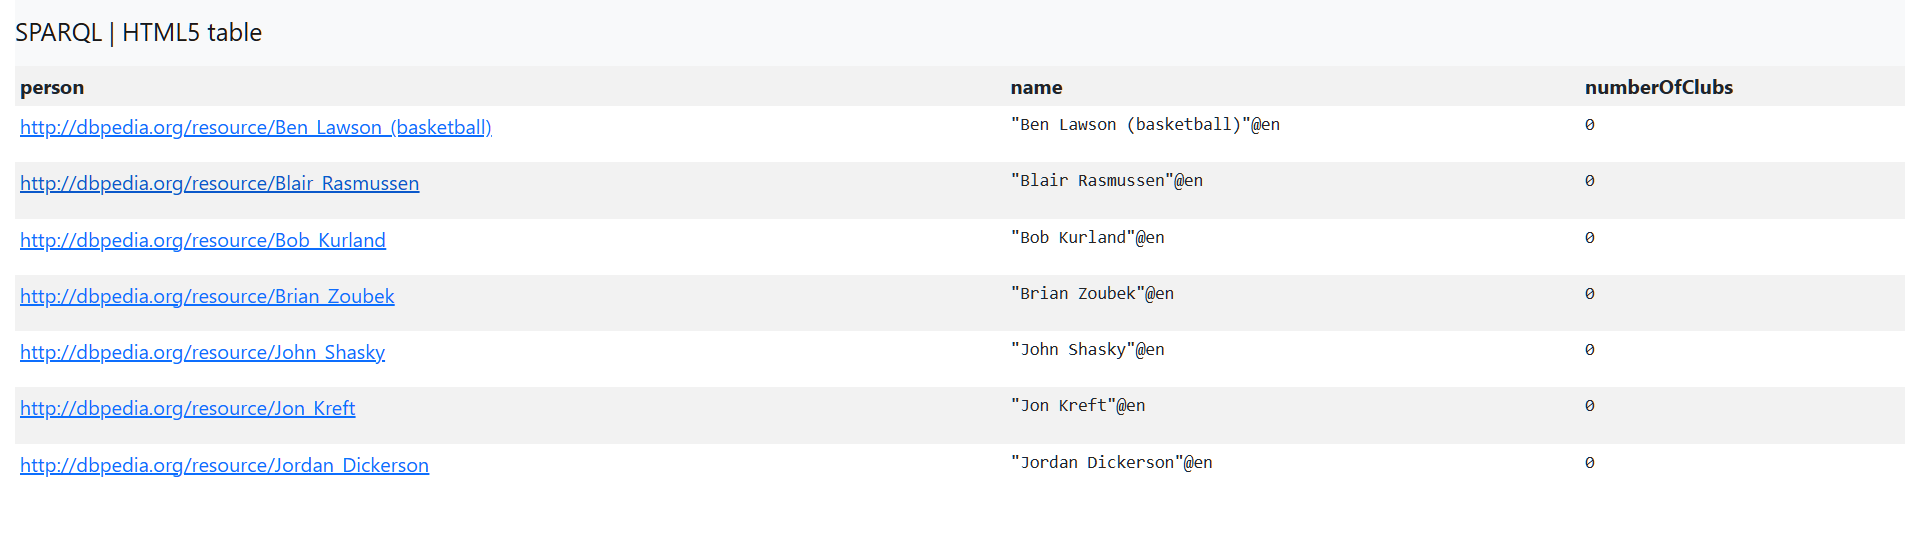
\includegraphics[width=\textwidth]{screenshots/Query3.png}
    \caption{Results of Query 3 executed on DBpedia Snorql}
    \label{fig:query3_results}
\end{figure}

\begin{table}[H]
    \centering
    \caption{Persons by height/weight and number of associated clubs}
    \label{tab:query3_results}
    \resizebox{\linewidth}{!}{%
    \begin{tabular}{|l|l|c|}
        \hline
        \textbf{Person URI} & \textbf{Name} & \textbf{Number of Clubs} \\
        \hline
        \url{http://dbpedia.org/resource/Ben_Lawson_(basketball)} & Ben Lawson (basketball) & 0 \\
        \url{http://dbpedia.org/resource/Blair_Rasmussen} & Blair Rasmussen & 0 \\
        \url{http://dbpedia.org/resource/Bob_Kurland} & Bob Kurland & 0 \\
        \url{http://dbpedia.org/resource/Brian_Zoubek} & Brian Zoubek & 0 \\
        \url{http://dbpedia.org/resource/John_Shasky} & John Shasky & 0 \\
        \url{http://dbpedia.org/resource/Jon_Kreft} & Jon Kreft & 0 \\
        \url{http://dbpedia.org/resource/Jordan_Dickerson} & Jordan Dickerson & 0 \\
        \hline
    \end{tabular}
    }% end resizebox
\end{table}



\subsubsection{Results Analysis}

This advanced query demonstrates:

\begin{itemize}
    \item \textbf{Aggregation functions:} COUNT to count relationships
    \item \textbf{Optional patterns:} OPTIONAL to handle missing data
    \item \textbf{Logical operators:} UNION for alternative conditions
    \item \textbf{Grouping:} GROUP BY for entity-based analysis
    \item \textbf{Custom ordering:} ORDER BY with explicit direction
\end{itemize}

The results likely include professional athletes (basketball, American football) given the physical characteristics. The number of clubs may indicate career mobility.

%==============================================================================
% SECTION 4: CONCLUSIONS
%==============================================================================
\section{Conclusions}

\subsection{Learnings about Ontologies}

Through this practice, fundamental knowledge has been acquired about:

\begin{itemize}
    \item \textbf{Ontology structure:} Understanding of class hierarchy, properties, and relationships
    \item \textbf{Knowledge modeling:} Ability to formally represent real-world concepts
    \item \textbf{Axioms and restrictions:} Use of descriptive logic to express semantic relationships
    \item \textbf{TBox vs ABox:} Distinction between terminology (classes) and assertions (instances)
    \item \textbf{Automated reasoning:} Understanding how reasoners can infer new knowledge
\end{itemize}

\subsection{Experience with WebProtégé}

WebProtégé proved to be a powerful tool for:

\begin{itemize}
    \item \textbf{Collaborative editing:} Accessible web interface without local installation
    \item \textbf{Visualization:} Entity graphs that facilitate understanding of relationships
    \item \textbf{Change management:} Complete history of modifications
    \item \textbf{Interoperability:} Import/export of standard formats (OWL)
\end{itemize}

\textbf{Difficulties encountered:}
\begin{itemize}
    \item Need to remove problematic import lines
    \item Learning curve in axiom syntax
    \item Management of existing properties vs. creating new ones
\end{itemize}

\subsection{Learnings about SPARQL}

SPARQL proved to be a powerful query language:

\begin{itemize}
    \item \textbf{Expressiveness:} Ability to formulate complex queries with multiple criteria
    \item \textbf{Functions:} Extensive library of functions for strings, numbers, dates, aggregation
    \item \textbf{Optional patterns:} Flexibility to handle incomplete data
    \item \textbf{Federation:} Possibility to query multiple endpoints
\end{itemize}

\textbf{Key concepts learned:}
\begin{itemize}
    \item Triple patterns as the basis of queries
    \item Importance of FILTERs to refine results
    \item Use of aggregation functions (COUNT, SUM, AVG, etc.)
    \item Logical operators (UNION, OPTIONAL, FILTER)
    \item Result ordering and limitation
\end{itemize}

\subsection{Practical Applications}

The acquired knowledge has applications in:

\begin{enumerate}
    \item \textbf{Food recommendation systems:}
    \begin{itemize}
        \item Suggest foods based on allergen restrictions
        \item Warn about potential risks
        \item Personalization according to health profiles
    \end{itemize}
    
    \item \textbf{Intelligent labeling:}
    \begin{itemize}
        \item Automation of nutritional labels
        \item Compliance with allergen regulations
        \item Ingredient traceability
    \end{itemize}
    
    \item \textbf{Public health analysis:}
    \begin{itemize}
        \item Correlation between diet and diseases
        \item Identification of epidemiological patterns
        \item Evidence-based health policies
    \end{itemize}
    
    \item \textbf{Semantic Web:}
    \begin{itemize}
        \item Integration of heterogeneous data
        \item Federated queries over multiple sources
        \item Linked Data applications
    \end{itemize}
\end{enumerate}

\subsection{Final Reflection}

Ontologies represent a fundamental tool for knowledge representation and management in intelligent systems. The combination of well-designed ontologies (such as OFFF) with expressive query languages (such as SPARQL) allows creating sophisticated applications that can reason about complex data and provide valuable information to users.

The practical experience with WebProtégé and DBpedia has provided a tangible understanding of theoretical concepts, demonstrating the viability and utility of Semantic Web technologies in real-world applications.

%==============================================================================
% REFERENCES
%==============================================================================
\section{References}

\begin{enumerate}
    \item Ding, Y., Pramanik, S., Muppala, S., et al. (2021). \textit{The ontology of fast food facts: conceptualization of nutritional fast food data for consumers and semantic web applications}. BMC Medical Informatics and Decision Making, 21, 275. \\
    \url{https://bmcmedinformdecismak.biomedcentral.com/articles/10.1186/s12911-021-01636-1}
    
    \item UTHealth Ontology. (2021). \textit{OFFF - Ontology of Fast Food Facts}. GitHub Repository. \\
    \url{https://github.com/UTHealth-Ontology/OFFF/}
    
    \item Wikipedia. (2025). \textit{List of allergens}. \\
    \url{https://en.wikipedia.org/wiki/List_of_allergens}
    
    \item Stanford University. (2025). \textit{WebProtégé: A Free, Open-Source Ontology Editor}. \\
    \url{https://webprotege.stanford.edu/}
    
    \item DBpedia Association. (2025). \textit{DBpedia SPARQL Endpoint}. \\
    \url{https://dbpedia.org/sparql/}
    
    \item DBpedia Association. (2025). \textit{DBpedia Snorql - SPARQL Query Interface}. \\
    \url{https://dbpedia.org/snorql/}
    
    \item W3C. (2013). \textit{SPARQL 1.1 Query Language}. W3C Recommendation. \\
    \url{https://www.w3.org/TR/sparql11-query/}
    
    \item W3C. (2012). \textit{OWL 2 Web Ontology Language Document Overview (Second Edition)}. W3C Recommendation. \\
    \url{https://www.w3.org/TR/owl2-overview/}
    
    \item Horrocks, I., Patel-Schneider, P. F., \& van Harmelen, F. (2003). \textit{From SHIQ and RDF to OWL: The making of a web ontology language}. Journal of Web Semantics, 1(1), 7-26.
    
    \item Bizer, C., Heath, T., \& Berners-Lee, T. (2009). \textit{Linked Data - The Story So Far}. International Journal on Semantic Web and Information Systems, 5(3), 1-22.
\end{enumerate}

%==============================================================================
% APPENDICES
%==============================================================================
\newpage
\appendix

\section{Modified Ontology File}

The modified ontology is found in the file \texttt{offf\_modified.owl} delivered together with this report.

\subsection{Modification Summary}

\begin{itemize}
    \item \textbf{Classes added:} 12 (10 allergens + Allergy + Inflammation)
    \item \textbf{Relationships added:} 14 causal axioms
    \item \textbf{Individuals added:} 1 (My fish sandwich)
    \item \textbf{Data properties:} 2 assigned values
\end{itemize}

\section{Complete SPARQL Code}

All SPARQL query files are found in the \texttt{sparql\_queries/} folder:

\begin{itemize}
    \item \texttt{query1\_artists.sparql} - Artists starting with ``Mado''
    \item \texttt{query2\_persons\_height.sparql} - Persons by height and birth date
    \item \texttt{query3\_persons\_clubs.sparql} - Persons by height/weight and number of clubs
\end{itemize}

\section{Additional Screenshots}

All screenshots include the username \texttt{santi\_david} from WebProtégé to validate authorship of the work.

\subsection{Screenshot List}

\begin{enumerate}
    \item \texttt{Allergens.png} - Allergen hierarchy
    \item \texttt{allergy.png} - Allergy class
    \item \texttt{inflammation\_1.png} - Relationship with Heart Disease
    \item \texttt{inflammation\_2.png} - Relationship with Hypertension
    \item \texttt{inflammation\_3.png} - Relationship with Obesity
    \item \texttt{inflammation\_4.png} - Relationship with Type II Diabetes
    \item \texttt{My fish sandwich.png} - Individual with data properties
    \item \texttt{Query1.png} - Query 1 results
    \item \texttt{Qiery2.png} - Query 2 results
    \item \texttt{Query3.png} - Query 3 results
\end{enumerate}

%==============================================================================
% END OF DOCUMENT
%==============================================================================
\end{document}
